% !TeX spellcheck = es_ES
\documentclass[11pt,a4paper,twoside]{report}

% ===== Paquetes esenciales =====
\usepackage[spanish]{babel}
\usepackage[utf8]{inputenc}
\usepackage[T1]{fontenc}
\usepackage{lmodern}
\usepackage{setspace}
\usepackage{hyperref}
\usepackage{fancyhdr}
\usepackage{graphicx}
\usepackage{geometry}
\usepackage{tocloft}
\usepackage{titlesec}
\usepackage{listings}
\usepackage{xcolor}
\usepackage{float}
\usepackage{url}
\usepackage{tikz}
\usepackage{courier}
\usepackage{pgfgantt}
\usepackage{enumitem}
\usepackage{placeins}
\usepackage{tocloft}
\usepackage{subcaption}
\usepackage{pdfpages}
\usepackage{tabularx}
\usepackage{array}
\usetikzlibrary{shapes, arrows, positioning}
\usepackage[spanish]{babel}

\addto\captionsspanish{%
	\renewcommand{\tablename}{Tabla}
	\renewcommand{\listtablename}{Índice de tablas}
}

\renewcommand{\lstlistlistingname}{Índice de Códigos}

\raggedbottom

\titlespacing*{\subsection}{0pt}{1em}{0.5em}

% ===== Configuraciones generales =====
\setlength{\headheight}{16pt}
\geometry{left=25mm, right=25mm, top=25mm, bottom=25mm}
\linespread{1.15} % Interlineado normativo

% ===== Encabezado y pie de página =====
\pagestyle{fancy}
\fancyhf{}
\fancyhead[LE,RO]{\leftmark}
\fancyfoot[CE,CO]{\thepage}

% ===== Formato de títulos =====
\titleformat{\chapter}[hang]{\bfseries\huge}{\thechapter.}{1pc}{}
\titlespacing*{\chapter}{0pt}{-10pt}{20pt}
\titleformat{\section}[hang]{\bfseries\Large}{\thesection.}{1pc}{}
\titleformat{\subsection}[hang]{\bfseries\large}{\thesubsection.}{1pc}{}
\renewcommand{\cftchapleader}{\cftdotfill{\cftdotsep}}

% Definición de colores si aún no los has puesto
\definecolor{mygreen}{rgb}{0,0.6,0}
\definecolor{mygray}{rgb}{0.5,0.5,0.5}
\definecolor{mymauve}{rgb}{0.58,0,0.82}

% Estilo snortstyle completo y compatible
% Estilo snortstyle completo y compatible
\lstdefinestyle{snortstyle}{
	backgroundcolor=\color{white},
	basicstyle=\footnotesize\ttfamily,
	breakatwhitespace=false,
	breaklines=true,
	captionpos=b,
	commentstyle=\color{mygreen},
	escapeinside={\%*}{*)},
	extendedchars=true,
	frame=single,
	keepspaces=true,
	keywordstyle=\color{blue},
	language=bash,
	morekeywords={sudo,systemctl,make,cmake,apt,tar,configure},
	numbers=left,
	numbersep=5pt,
	numberstyle=\tiny\color{mygray},
	rulecolor=\color{black},
	showspaces=false,
	showstringspaces=false,
	showtabs=false,
	stepnumber=2,
	stringstyle=\color{mymauve},
	tabsize=2,
	postbreak=\mbox{\textcolor{red}{$\hookrightarrow$}\space},
	title=\lstname,
	literate=
	{á}{{\'a}}1 {é}{{\'e}}1 {í}{{\'i}}1 {ó}{{\'o}}1 {ú}{{\'u}}1
	{Á}{{\'A}}1 {É}{{\'E}}1 {Í}{{\'I}}1 {Ó}{{\'O}}1 {Ú}{{\'U}}1
	{ñ}{{\~n}}1 {Ñ}{{\~N}}1 {¿}{{?`}}1 {¡}{{!`}}1
	{°}{{\textdegree}}1 {→}{{$\rightarrow$}}1 {⇒}{{$\Rightarrow$}}1
	{≥}{{$\geq$}}1 {≤}{{$\leq$}}1 {–}{{--}}1
	{“}{{``}}1 {”}{{''}}1 {’}{{'}}1 {•}{{\textbullet}}1
	{\{}{{\{}}1 {\}}{{\}}}1
	{\_}{{\_}}1 {\%}{{\%}}1 {\$}{{\$}}1
	{\\}{{\textbackslash}}1 {\#}{{\#}}1 {\&}{{\&}}1
	{\^}{{\^{}}}1 {\~}{{\~{}}}1 {\|}{{\textbar}}1
	{\033}{{\textbackslash033}}1,
}

% Activar el estilo globalmente
\lstset{style=snortstyle}

\lstdefinestyle{commandstyle}{
	backgroundcolor=\color{gray!10},
	basicstyle=\ttfamily\small\color{black}, % Todo el texto en negro
	frame=single,
	breaklines=true,
	showstringspaces=false,
	columns=flexible,
	xleftmargin=1.5em,
	framexleftmargin=1.5em,
	stringstyle=\color{mymauve}, % Cadenas en rosado
	commentstyle=\color{mygreen}, % Comentarios (si los hay)
	keywordstyle=\color{black}, % Keywords en negro (elimina el azul)
	language=bash,
	numbers=left,
	numberstyle=\tiny\color{gray},
	numbersep=8pt,
	firstnumber=1,
	stepnumber=1,
	numberblanklines=false,
	numberfirstline=true,
	prebreak=\mbox{\textcolor{red}{$\hookleftarrow$}\space},
	postbreak=\mbox{\textcolor{red}{$\hookrightarrow$}\space},
	morekeywords={} % Vaciamos completamente la lista de keywords
}

% Para evitar que \lstlistoflistings añada al TOC
\makeatletter
\let\oldlstlistoflistings\lstlistoflistings
\renewcommand{\lstlistoflistings}{\begingroup\let\addcontentsline\@gobble\oldlstlistoflistings\endgroup}
\makeatother

% Título en español para el índice de códigos
\renewcommand{\lstlistlistingname}{Índice de Códigos}


% ===== Inicio del documento =====
\begin{document}
	
	\pagenumbering{roman}
	
	% ===== Portada (debes sustituirla por la oficial del Anexo II en la entrega) =====
\cleardoublepage
\includepdf[pages=1, pagecommand={\thispagestyle{empty}}, fitpaper=true]{portada.pdf}
	
	\thispagestyle{empty}
	\cleardoublepage
	\thispagestyle{empty}
	
	
	
	% ===== Licencia Creative Commons =====
	\newpage
	\thispagestyle{empty}
	\begin{center}
		\vspace*{\fill}
		\includegraphics[width=0.3\textwidth]{adicional/cc.xlarge.png}\\
		Este trabajo está bajo una licencia Creative Commons Atribución-NoComercial-CompartirIgual 4.0 Internacional.
		\vspace*{\fill}
	\end{center}
	
	\newpage
	\thispagestyle{empty}
	\null
	\newpage
	
	% ===== Agradecimientos =====
	\cleardoublepage
	\thispagestyle{empty}
	{
		\begin{center}
			\Large\bfseries Agradecimientos
		\end{center}
		
		\vspace{1cm}
		
		Quiero expresar mi más sincero agradecimiento a mi tutor, Julio Gómez López, y a mi cotutor, Nicolás Padilla Soriano, por su orientación y apoyo durante
		todo el desarrollo de este trabajo. Su experiencia ha sido el pilar para mantener un enfoque de este proyecto.\newline
		
		También quiero dar las gracias a mi familia, en especial a mis padres, por haberme transmitido desde pequeño el valor del esfuerzo, la constancia y la curiosidad.
	    Su confianza incondicional me ha permitido perseguir mis metas con libertad y determinación.\newline
		
		A mis amigos y compañeros de carrera, con quienes he compartido frustraciones, risas, noches de trabajo y logros, gracias por formar parte de este camino.
		Vuestra compañía ha sido tan importante como el contenido aprendido.\newline
		
		Y por último, a mí mismo, por no rendirme. Por seguir adelante incluso cuando el cansancio o la duda amenazaban con paralizarme. Este trabajo representa no
		solo un proyecto académico, sino también un ejercicio de crecimiento, disciplina y pasión por la tecnología como herramienta para construir un mundo más seguro y accesible.
		
		\vfill
	}
	
		\newpage
	\thispagestyle{empty}
		\cleardoublepage

	% ===== Índice general =====
	\tableofcontents
	\newpage
	
	% ===== Índice de figuras =====
	\listoffigures
	\newpage
	
	% ===== Índice de tablas/cuadros =====
	\listoftables
	
	% SOLO esto para insertar página vacía después
	\newpage
	\thispagestyle{empty}
	\null
	\newpage
	
% ===== Índice de códigos (sin TOC pero con encabezado) =====
% ===== Índice de códigos =====
\cleardoublepage
\markboth{Índice de Códigos}{Índice de Códigos}
\lstlistoflistings


% ===== Abreviaturas (sin TOC pero con encabezado) =====
\chapter*{Abreviaturas}
\markboth{Abreviaturas}{Abreviaturas}
\begin{itemize}
	\item \textbf{APT}: (Advanced Persistent Threat). Amenaza Avanzada Persistente. Suele involucrar ataques dirigidos y prolongados contra objetivos concretos.
	\item \textbf{ClamAV}: Antivirus de código abierto que analiza y detecta archivos maliciosos o infecciones. Se integra como complemento en el proyecto.
	\item \textbf{CPU}: (Central Processing Unit). Unidad central de procesamiento, comúnmente conocida como procesador, encargada de ejecutar instrucciones en un sistema.
	\item \textbf{CSV}: (Comma-Separated Values). Formato de archivo de texto plano que representa datos tabulares separados por comas o puntos y coma.
	\item \textbf{Debian Package (*.deb)}: Formato estándar de paquetes en sistemas GNU/Linux basados en Debian/Ubuntu. Facilita la instalación y gestión de software.
	\item \textbf{DoS}: (Denial of Service). Ataque que busca interrumpir el funcionamiento normal de un sistema o red.
	\item \textbf{FTP}: (File Transfer Protocol). Protocolo para la transferencia de archivos en redes IP.
	\item \textbf{GNU/Linux}: Sistema operativo de software libre en el que se basan distribuciones como Ubuntu, Debian, CentOS, etc.
	\item \textbf{HIDS}: (Host Intrusion Detection System). Sistema de Detección de Intrusiones basado en Host, centrado en vigilar el comportamiento interno de un equipo específico.
	\item \textbf{HTTP}: (Hypertext Transfer Protocol). Protocolo de comunicación utilizado en la web para transmitir información entre cliente y servidor.
	\item \textbf{HTTP2}: Segunda versión del protocolo HTTP, optimizada para mayor velocidad y eficiencia.
	\item \textbf{ICMP}: (Internet Control Message Protocol). Protocolo usado para enviar mensajes de error y diagnóstico en redes IP.
	\item \textbf{IDS}: (Intrusion Detection System). Sistema de Detección de Intrusiones (término general). Comprende tanto la detección en host (HIDS) como en red (NIDS).
	\item \textbf{IEC 104}: Protocolo de comunicación utilizado en sistemas de automatización industrial y redes eléctricas.
	\item \textbf{IMAP}: (Internet Message Access Protocol). Protocolo para acceder y gestionar correos electrónicos en servidores remotos.
	\item \textbf{IPS}: (Intrusion Prevention System). Sistema de Prevención de Intrusiones. Además de detectar acciones maliciosas, reacciona automáticamente para bloquearlas.
	\item \textbf{LuaJIT}: Implementación just-in-time (JIT) del lenguaje de scripting Lua, que Snort 3 utiliza para reglas y configuraciones más flexibles.
	\item \textbf{MIME}: (Multipurpose Internet Mail Extensions). Estándar para enviar contenido diverso (como archivos) a través de correos electrónicos.
	\item \textbf{NIDS}: (Network Intrusion Detection System). Sistema de Detección de Intrusiones en Red. Se encarga de monitorear el tráfico que circula por la red en busca de acciones sospechosas o maliciosas.
	\item \textbf{OT}: (Operational Technology). Tecnología usada para controlar procesos físicos en industrias, como sistemas SCADA o PLCs.
	\item \textbf{POP3}: (Post Office Protocol version 3). Protocolo usado para recuperar correos electrónicos desde un servidor.
	\item \textbf{Raspberry Pi (R-Pi)}: Máquina de bajo coste y tamaño reducido. Muy popular para proyectos de electrónica, servidores ligeros.
	\item \textbf{R-SNORT}: Adaptación o paquete de Snort diseñado para ejecutarse de forma optimizada en una Raspberry Pi, con funciones específicas para redes SOHO.
	\item \textbf{SIEM}: (Security Information and Event Management). Plataforma que recopila y correlaciona datos de seguridad (logs, alertas, eventos) para proporcionar una visión global y centralizada.
	\item \textbf{SIP}: (Session Initiation Protocol). Protocolo usado principalmente para establecer y controlar sesiones multimedia, como llamadas VoIP.
	\item \textbf{SMB}: (Server Message Block). Protocolo de red para compartir archivos, impresoras y puertos serie entre nodos.
	\item \textbf{Snort}: Herramienta de código abierto usada para la detección de intrusiones en red, muy extendida en el ámbito de la ciberseguridad.
	\item \textbf{SOHO}: (Small Office/Home Office). Redes pequeñas o domésticas, típicas de oficinas y hogares con recursos más limitados que una gran empresa.
	\item \textbf{SSL/TLS}: (Secure Sockets Layer / Transport Layer Security). Protocolos de cifrado que permiten la comunicación segura entre sistemas a través de redes.
\end{itemize}

% Introducción
\cleardoublepage
\chapter*{Introducción}
\addcontentsline{toc}{chapter}{Introducción}
\markboth{Introducción}{Introducción}
\pagenumbering{arabic}
\setcounter{secnumdepth}{0} % ← NO numerar secciones temporalmente

La creciente dependencia digital de las empresas ha convertido a la ciberseguridad en un factor crítico para la supervivencia y éxito de cualquier negocio, especialmente en el caso de las pequeñas y medianas empresas (PYMEs). En España, donde las PYMEs constituyen la base del tejido empresarial (en torno al 99\% de las empresas) \cite{enisa2023}
, los ciberataques se han disparado en número y sofisticación. Se estima que casi la mitad de los ciberataques a nivel mundial van dirigidos a PYMEs, un problema particularmente serio en países como España \cite{google2024}. De hecho, siete de cada diez ataques en España tienen como objetivo organizaciones de tamaño pequeño o mediano, aprovechando que suelen contar con menos medidas de seguridad y sistemas más vulnerables. Las consecuencias de estas brechas pueden ser devastadoras: según datos de Telefónica, un 60\% de las PYMEs que sufren un ciberataque acaban desapareciendo en menos de seis meses tras el incidente \cite{telefonica2023}, ya sea por pérdidas financieras, daños reputacionales o interrupción prolongada de sus operaciones. Este panorama pone de manifiesto la importancia de una ciberseguridad robusta para la supervivencia empresarial en la era digital.\newline

Sin embargo, lograr una protección adecuada presenta desafíos particulares para las PYMEs. Estas organizaciones suelen enfrentar amenazas diversas desde campañas de phishing y malware hasta ransomware y ataques dirigidos a sus aplicaciones web pero carecen de los recursos financieros y técnicos que disponen las grandes corporaciones para contrarrestarlas. En general, muchas PYMEs son especialmente vulnerables, ya que “afrontan retos digitales con recursos limitados y, en ocasiones, con desconocimiento de las amenazas que conllevan”. La falta de personal especializado en seguridad, junto con presupuestos exiguos, deriva en lagunas importantes de protección: no siempre se monitoriza la red en busca de comportamientos anómalos, no se cuenta con mecanismos sólidos de detección de intrusiones, y la prevención de fugas de información suele quedar relegada o confiada únicamente a medidas básicas. Todo ello ocurre en un contexto donde los ataques no solo van en aumento (INCIBE gestionó 107.500 incidentes en 2022, un 15\% más que el año anterior), sino que además los incidentes críticos están creciendo exponencialmente, poniendo en riesgo la continuidad del negocio.\newline

En respuesta a esta problemática, organismos e iniciativas tanto nacionales como europeas han comenzado a centrar su atención en las PYMEs. La Unión Europea, consciente del papel fundamental de estas empresas en la economía, ha incluido a muchas de ellas dentro del alcance de la nueva Directiva NIS2 para reforzar su ciberresiliencia \cite{incibe2025}. En España, instituciones como INCIBE impulsan programas de sensibilización y apoyo específico (Protege tu Empresa, Kit Digital, ayudas de Activa Ciberseguridad, etc.), reconociendo que la ciberseguridad de las PYMEs es un asunto de interés general. No obstante, sigue existiendo una brecha importante entre las necesidades de seguridad de las PYMEs y las soluciones disponibles en el mercado que puedan permitirse o gestionar sin un departamento técnico dedicado.\newline

En este Trabajo Fin de Grado se plantea abordar dicha brecha. La idea central es explorar y justificar la viabilidad de una solución accesible, profesional y asequible basada en Snort 3 sobre una plataforma de bajo coste (Raspberry Pi), complementada con una interfaz web de gestión y paneles visuales de Grafana –una solución que denominaremos R-Snort– para cubrir las necesidades actuales de ciberseguridad de las PYMEs españolas. En los siguientes apartados se detallarán la motivación y objetivos concretos del proyecto, así como un análisis del estado del arte y de los requerimientos de seguridad más apremiantes para este sector empresarial.

% Capítulos
\section{Motivación}

La motivación de este proyecto surge de la constatación de una necesidad real y urgente: las pequeñas y medianas empresas se encuentran en la mira de los ciberdelincuentes, pero no disponen de las herramientas ni conocimientos adecuados para protegerse. A pesar de ser blanco de la mayoría de ataques, muchas PYMEs en España aún “no cuentan con el presupuesto suficiente para hacer frente a los ciberataques”, y más preocupante incluso, carecen de concienciación y conocimiento sobre las soluciones a su alcance. Expertos en seguridad señalan que esta falta de concienciación es un factor crítico –en ocasiones mayor obstáculo que el económico–, pues existen medidas de bajo coste que podrían mitigar gran parte de las amenazas si las empresas supieran cómo aplicarlas. En otras palabras, el problema no es solo qué falta de recursos, sino también falta de accesibilidad a soluciones de ciberseguridad adaptadas a las limitaciones de las PYMEs.\newline

Actualmente, las opciones profesionales en el mercado para monitorizar redes, prevenir fugas de datos o detectar intrusiones suelen implicar costosas inversiones en equipos especializados, licencias de software o servicios gestionados (firewalls de nueva generación, sistemas de prevención de intrusiones, plataformas SIEM, etc.). Estas soluciones están pensadas para empresas con departamentos de TI consolidados y con presupuesto holgado, lo que deja a las PYMEs en una situación de desventaja: o bien operan sin las debidas medidas de seguridad (asumiendo riesgos elevados), o intentan implementar herramientas gratuitas/open-source por su cuenta, encontrándose con dificultades técnicas de configuración y mantenimiento. Por ejemplo, Snort –un sistema de detección de intrusiones de código abierto ampliamente reconocido– requiere experiencia para su despliegue y gestión, lo que suele exceder las capacidades del personal de TI generalista con el que cuentan las PYMEs típicas. De igual modo, soluciones de prevención de fuga de información o monitorización de red continua se perciben como complejas y fuera del alcance práctico de estas organizaciones.\newline

Este TFG nace con la motivación de democratizar el acceso a la ciberseguridad para las PYMEs, aprovechando herramientas open-source de probada eficacia pero integrándolas en una plataforma que minimice las barreras de entrada. La elección de una Raspberry Pi como base responde al objetivo de abaratar costes de hardware al máximo, a la vez que proporciona la flexibilidad de un entorno Linux completo. Snort 3 se adopta por ser la evolución moderna de uno de los IDS más fiables a nivel industrial, ahora con mejoras de rendimiento y usabilidad que lo hacen más adaptable a entornos modestos. Al desarrollar una interfaz web amigable y complementarla con la visualización de datos mediante Grafana, buscamos que la solución resultante R-Snort sea utilizable por administradores no especializados, permitiéndoles vigilar el tráfico de su red, recibir alertas de intrusiones o comportamientos sospechosos, y supervisar potenciales fugas de información de forma sencilla e intuitiva.\newline

En resumen, la motivación del proyecto se sustenta en tres pilares: (1) la necesidad palpable de mejorar la seguridad en PYMEs ante el aumento de amenazas, (2) la oportunidad de combinar tecnología open-source y hardware económico para crear una herramienta adaptada a dichas necesidades, y (3) la convicción de que una solución accesible y de bajo coste puede marcar la diferencia evitando incidentes que podrían suponer el cierre de muchas pequeñas empresas. Atendiendo a esta motivación, a continuación se definen los objetivos concretos que se pretenden alcanzar.

\section{Objetivos}

El objetivo general de este Trabajo Fin de Grado es diseñar, implementar y validar un sistema integral de monitorización y detección de intrusiones orientado a PYMEs, basado en Snort 3 sobre Raspberry Pi (R-Snort), con interfaz web de gestión y visualización mediante Grafana, que responda eficazmente a las necesidades de seguridad de este tipo de organizaciones.\newline

De este objetivo principal se desprenden los siguientes objetivos específicos:

\begin{enumerate}
	\item Analizar las necesidades de ciberseguridad de las PYMEs en España, particularmente en los ámbitos de monitorización de red, prevención de fugas de información y detección de intrusiones, así como sus limitaciones presupuestarias y técnicas. Este análisis, sustentado en la revisión del estado del arte y fuentes especializadas, servirá para justificar los requisitos y el enfoque de la solución propuesta.
	
	\item Diseñar la arquitectura de R-Snort, seleccionando los componentes adecuados (hardware Raspberry Pi y software Snort 3, junto con herramientas de apoyo como motores de almacenamiento de logs, dashboards de Grafana, etc.) y configurando una instancia optimizada de Snort que pueda funcionar de forma estable y eficiente en un entorno de recursos limitados. Esto implica ajustar la carga de reglas, parámetros de rendimiento y posibles complementos para asegurar que la Raspberry Pi pueda analizar el tráfico en tiempo real sin degradación notable.
	
	\item Desarrollar una interfaz web intuitiva para la gestión de Snort y la visualización de eventos de seguridad. La interfaz deberá permitir realizar las tareas más comunes (por ejemplo, actualizar reglas, iniciar/detener la captura de tráfico, revisar alertas) sin necesidad de recurrir a la línea de comandos, haciendo la solución más accesible a personal no experto. Asimismo, se integrará Grafana u otro sistema de visualización para presentar métricas e indicadores de la red (p. ej., volumen de tráfico, alertas por tipo, tendencias temporales) de forma gráfica y comprensible.
	
	\item Validar el sistema R-Snort en un escenario representativo de PYME, verificando que cumple con los requisitos identificados. Esto incluirá pruebas de funcionalidad (comprobando que detecta intrusiones conocidas, que registra eventos de posible exfiltración de datos, etc.), de rendimiento (medir el tráfico máximo que puede manejar la Raspberry Pi con Snort 3 y el impacto en tiempos de respuesta), y de usabilidad (evaluar si un usuario con conocimientos técnicos básicos puede manejar la interfaz y entender la información proporcionada). Los resultados de esta validación permitirán determinar en qué medida la solución efectivamente mejora la postura de seguridad de una PYME típica y qué limitaciones o consideraciones deben tenerse en cuenta en su despliegue real.
\end{enumerate}

Con estos objetivos, se pretende que el TFG no solo culmine en un prototipo funcional, sino también en una justificación bien fundamentada de por qué dicha solución es adecuada para las PYMEs y cómo contribuye a cerrar la brecha existente entre los riesgos que enfrentan y los medios de protección actualmente a su disposición.


\section{Fases de la realización y cronograma}
en proceso
\section{Estructura y metodología}
en proceso

\setcounter{secnumdepth}{2} 

\cleardoublepage
\thispagestyle{empty}
\chapter{Sistemas de detección de intrusos: Snort y frontends}

\section{IDS / NIDS}

Un \textit{Intrusion Detection System} (IDS), o sistema de detección de intrusos, es una herramienta de seguridad cuya función principal es identificar accesos no autorizados o comportamientos anómalos en un sistema o red informática \cite{wikiNIDS}. Estos sistemas analizan los eventos de la red o del host en tiempo real buscando patrones que puedan indicar amenazas, como ataques de denegación de servicio, escaneos de puertos o intentos de intrusión \cite{NISTSP80094}. En general, un IDS no actúa directamente sobre el tráfico; se limita a monitorear y generar alertas para notificar a los administradores cuando detecta actividades sospechosas o violaciones a las políticas de seguridad.\newline

Existen dos grandes categorías de IDS según el ámbito que vigilan: los basados en host (HIDS) y los basados en red (NIDS). Un HIDS se despliega en un equipo específico y analiza los registros (\textit{logs}) y actividades de ese sistema para descubrir intrusiones locales (por ejemplo, modificaciones no autorizadas, accesos indebidos, etc.). Por otro lado, un \textit{Network IDS} o NIDS inspecciona el tráfico de una red completa o segmento de red para detectar amenazas que transitan por ella. El NIDS examina todos los paquetes que atraviesan la red en tiempo real, buscando en ellos patrones o firmas conocidas de ataques (malware, \textit{port scanning}, explotación de vulnerabilidades, etc.) y puede detectar tanto tráfico malicioso entrante como saliente. Debido a su naturaleza pasiva (escucha en modo promiscuo una copia del tráfico), un NIDS no introduce prácticamente latencia ni altera el flujo de datos en la red que vigila.\newline

Es importante distinguir un IDS de un sistema de prevención de intrusos o IPS (\textit{Intrusion Prevention System}). La diferencia clave es que el IDS opera de forma pasiva (detectando y alertando sobre posibles ataques), mientras que un IPS actúa de forma activa/intervencionista: un IPS posee todas las capacidades de detección de un IDS pero, adicionalmente, puede bloquear o impedir automáticamente el tráfico malicioso una vez identificado \cite{a2secure2019}. En otras palabras, el IDS avisa de una intrusión, pero es el administrador quien debe tomar acciones (por ejemplo, actualizar reglas de cortafuegos o aislar equipos comprometidos); en cambio, un IPS está situado en línea en la red y, al detectar un ataque, puede descartarlo o cortarlo en el momento. Por este motivo, a menudo se habla de sistemas IDPS (detección y prevención) cuando una misma solución combina ambas facetas.\newline

Diversos ejemplos ilustran cada tipo de sistema. En el ámbito de host (HIDS) se pueden citar soluciones como OSSEC, Wazuh o Samhain, que monitorizan archivos de log y actividades de un servidor específico. En el ámbito de red (NIDS), destacan herramientas de código abierto ampliamente utilizadas como Snort, Suricata o Bro/Zeek. En particular, Snort se ha convertido en el estándar de facto con el que se comparan todos los IDS de red desde hace más de dos décadas \cite{SnortBlog2011}. Snort es un NIDS (y IPS) open source que emplea un conjunto actualizado de \textit{reglas} de detección para identificar patrones de tráfico malicioso; cuando un paquete o flujo coincide con alguna firma o criterio definido en sus reglas, Snort genera una alerta que notifica del posible incidente \cite{CiscoSnort3Blog}. Además, Snort puede desplegarse en modo \textit{inline} (en línea) actuando como IPS, de forma que no solo detecte sino que también bloquee aquellos paquetes que violen las reglas de seguridad. Esta versatilidad ha hecho que Snort sea una referencia obligada en IDS de red tanto para uso personal como empresarial, contando con una amplia comunidad que contribuye con reglas, mejoras y soporte.\newline


\section{R-Snort}

R-Snort es la denominación del sistema desarrollado en este proyecto, el cual consiste en una solución integral de monitorización y detección de intrusos basada en Snort 3 sobre hardware de bajo coste (una plataforma Raspberry Pi). En esencia, R-Snort implementa un sensor NIDS autónomo que aprovecha las mejoras de la nueva generación de Snort junto con una interfaz web para la gestión y visualización remota de eventos. A diferencia de un IDS tradicional aislado, R-Snort se concibe de forma modular con componentes que automatizan la recolección de datos, el análisis y la presentación de la información de seguridad, todo ello utilizando únicamente tecnologías abiertas.\newline

El \textbf{núcleo de detección} de R-Snort lo constituye Snort 3 ejecutándose en una Raspberry Pi. Snort 3 (también conocido como Snort++) es una reimplementación modernizada del motor Snort que aporta importantes ventajas técnicas respecto a la rama 2.X. Por ejemplo, Snort 3 fue reescrito en C++ para lograr una base de código más modular y fácil de mantener. Incorpora soporte nativo de multiproceso (hilos) y uso de memoria compartida, permitiendo explotar mejor los procesadores multi-núcleo y ofreciendo mayor rendimiento y escalabilidad en la inspección de tráfico. Asimismo, Snort 3 introduce un sistema flexible de complementos (\textit{plugins}) e integración con el lenguaje Lua (LuaJIT) para extender sus funcionalidades, por ejemplo añadiendo nuevas opciones de reglas o analizadores de protocolos de forma más sencilla que antes. La sintaxis de las reglas de detección también se refinó para hacerlas más concisas y fáciles de escribir, reduciendo partes innecesarias y optimizando la velocidad de evaluación \cite{Sakura2020}. Todas estas mejoras hacen de Snort 3 un motor más adaptable, eficiente y potente para nuestro sistema de detección de intrusos.\newline

En R-Snort, Snort 3 actúa como sensor de red, inspeccionando el tráfico (por ejemplo, mediante una interfaz en modo promiscuo o conectado a un puerto espejo de switch) y generando alertas de intrusión en formato JSON. Dichas alertas son procesadas y almacenadas para su consulta mediante la capa de \textbf{back-end}, que está implementada con un servidor web desarrollado en Spring Boot (framework Java) siguiendo una arquitectura de API REST. Este servidor intermedia entre el sensor y la interfaz de usuario, proporcionando servicios como el registro de alertas en una base de datos, la gestión de las reglas activas, y la exposición de endpoints seguros para que los administradores consulten el estado del sistema o apliquen configuraciones de forma remota.\newline

La \textbf{interface web} o front-end de R-Snort se ha construido como una \textit{single-page application} moderna utilizando Angular (framework JavaScript/TypeScript). A través de esta webapp, accesible desde cualquier navegador, el usuario puede visualizar en tiempo real las alertas generadas por Snort, revisar estadísticas históricas, filtrar y buscar eventos por múltiples criterios, así como realizar tareas de administración del sensor (activar/desactivar reglas, reiniciar el servicio IDS, cargar actualizaciones, etc.). El diseño front-end se ha orientado a la simplicidad y claridad en la presentación de datos, inspirándose en las mejores prácticas de UX de aplicaciones de monitoreo.\newline

Para enriquecer la experiencia de monitorización, R-Snort integra además la plataforma \textbf{Grafana} como herramienta de visualización de datos de seguridad. Grafana es un software open source ampliamente utilizado para construir paneles de control interactivos, y en nuestro proyecto se emplea para generar gráficas y paneles personalizados a partir de los datos de alertas y métricas del IDS. Por ejemplo, se han creado dashboards que muestran el número de alertas por unidad de tiempo, la clasificación de las alertas por severidad o tipo de ataque, e incluso mapas de calor de IP de origen/destino más detectadas. Este enfoque sigue la línea de otras implementaciones de comunidad que utilizan Grafana para visualizar eventos de Snort (a menudo en conjunción con bases de datos de tiempo real como Elasticsearch/Graylog) \cite{GrafanaForum2020}. En R-Snort, Grafana se conecta al almacenamiento de alertas del back-end y permite tener, dentro de la misma solución, una vista gráfica y analítica de la seguridad de la red en tiempo real.\newline

En conjunto, R-Snort supone una propuesta de IDS/NIDS completo de bajo coste y código abierto. Combina el potente motor de detección de Snort 3 (sensor) con un ecosistema web moderno (Spring Boot/Angular en el servidor y cliente) y herramientas de visualización profesionales (Grafana) para proporcionar a pequeñas y medianas empresas una plataforma accesible para proteger sus redes. Toda la solución se despliega sobre hardware económico (una Raspberry Pi como nodo sensor), lo que reduce la barrera de entrada en términos de inversión. Pese a su sencillez de despliegue, el sistema mantiene un enfoque modular y escalable: cada componente (detección, almacenamiento, visualización, gestión) está desacoplado, permitiendo en el futuro reemplazar o ampliar funcionalidades (por ejemplo, agregar más sensores en varias ubicaciones reportando al mismo back-end, o incorporar nuevas fuentes de datos de seguridad). En resumen, R-Snort demuestra cómo es posible aprovechar tecnologías abiertas actuales para construir un IDS integrado, manejable vía web y orientado a entornos con recursos limitados, sin incurrir en los altos costes ni complejidad de soluciones comerciales tradicionales.


\section{Frontends más utilizados de Snort}

A lo largo de la evolución de Snort han surgido múltiples aplicaciones front-end para facilitar la gestión y análisis de las alertas generadas por este IDS. Estos frontends web proveen consolas gráficas donde los eventos de Snort pueden visualizarse, filtrarse y reportarse de forma más amigable que mediante los logs en texto plano. A continuación se describen algunos de los frontends históricos más populares asociados a Snort –como Snorby, BASE, Aanval, Sguil o Snort Report– incluyendo sus características principales, enfoques y limitaciones, para luego comparar sus conceptos con la propuesta de nuestro R-Snort.\newline

\textbf{BASE (Basic Analysis and Security Engine)} es uno de los frontales web clásicos para Snort. Nació como una continuación del proyecto anterior ACID (\textit{Analysis Console for Intrusion Databases}), el cual fue un pionero en proveer una interfaz web para consultar las alertas registradas por Snort en una base de datos. ACID, desarrollado a inicios de los 2000, quedó discontinuado alrededor de 2003 \cite{SnorbyHelpnet2010}, pero BASE retomó su código y lo mejoró, añadiendo nuevas funciones y compatibilidad con múltiples idiomas. Al igual que ACID, BASE está escrito en PHP y se apoya típicamente en un stack LAMP (Linux-Apache-MySQL-PHP): Snort vuelca las alertas en una base de datos relacional (por ejemplo MySQL) –usando para ello complementos como Barnyard2– y BASE ofrece consultas, gráficos básicos y gestión de alertas desde una página web dinámica. Durante muchos años, BASE fue la interfaz preferida por la comunidad, llegando a superar las 200.000 descargas. Entre sus fortalezas estaban la simplicidad de despliegue y su funcionalidad probada para navegación y búsqueda en los eventos (permitiendo ordenar por fecha, tipo de ataque, IP, etc., y ver detalles de cada alerta). Como limitaciones, al ser una herramienta concebida hace más de 15 años, su interfaz resulta poco moderna y no ofrece visualizaciones avanzadas; además depende de tecnologías y librerías ya obsoletas, lo que puede dificultar su instalación en entornos actuales. A pesar de planes para rediseñar BASE e incluso cambiar su formato de base de datos, el proyecto perdió ímpetu tras la salida de sus mantenedores originales y su desarrollo activo se ha ralentizado considerablemente.\newline

\textbf{Snort Report} es otra solución veterana, centrada en proporcionar informes rápidos del estado del IDS. Surgido alrededor de 2001, Snort Report se distribuía como un módulo adicional ligero para obtener “instantáneas” de las alertas más recientes y resumir la actividad de Snort en la red \cite{SnortReport2010}. A diferencia de BASE, que brinda múltiples vistas y filtros de análisis forense, Snort Report se enfocaba en la monitorización en tiempo real: presentaba en una pantalla principal un tablero con las alertas actuales (número de eventos, tipo más frecuente, origen de las últimas alarmas, etc.), permitiendo al administrador hacerse una idea inmediata de lo que estaba ocurriendo en su sensor IDS. Era una aplicación sencilla en PHP que leía directamente de la base de datos de Snort o de los archivos de log. Entre sus ventajas estaba la facilidad de uso y la mínima configuración necesaria. Sin embargo, también ofrecía menos profundidad analítica que otras herramientas (no tenía tantas opciones de búsqueda histórica o correlación) y con el tiempo fue quedando relegada en favor de frontends más completos. Aun así, para pequeñas implementaciones Snort Report fue útil por su simplicidad. Con el lanzamiento de Snort 2.x y la aparición de otros dashboards más sofisticados, Snort Report dejó de actualizarse regularmente y hoy en día se considera descontinuado.\newline

\textbf{Aanval} representa una aproximación distinta, orientada a entornos empresariales que buscaban una solución más completa de tipo SIEM integrando a Snort. Es un producto comercial (desarrollado por Tactical FLEX, Inc.) que desde 2003 ha ofrecido soporte para recoger y correlacionar eventos de Snort, Suricata y fuentes de logs generales (syslog) en una plataforma unificada \cite{AanvalWiki}. Aanval se caracteriza por una interfaz web propietaria bastante pulida, con dashboards personalizables, mapas de topologías, alertas en tiempo real y gestión centralizada de múltiples sensores Snort. A lo largo de sus numerosas versiones, ha incorporado funcionalidades avanzadas como: clasificación de eventos por categorías de ataque, generación de informes ejecutivos, alertamiento vía correo/SMS, e integración con herramientas externas (por ejemplo, ticketing de incidentes). En esencia, Aanval va más allá de un simple visor de alertas y se posiciona como un centro de operaciones de seguridad (\textit{Security Operations Center} simplificado) para quienes despliegan Snort. Entre sus fortalezas está la robustez y amplitud de características, así como su continuidad en el tiempo (es uno de los frontends para Snort con más larga trayectoria, con mantenimiento activo por más de 15 años). Su principal desventaja, desde la perspectiva de nuestro proyecto, es que no es software libre; si bien tuvo versiones gratuitas limitadas, la versión completa de Aanval es de pago, lo que supone una barrera para PYMEs con presupuesto reducido. Asimismo, su enfoque todo-en-uno puede resultar complejo de desplegar en escenarios muy pequeños. No obstante, conceptualmente Aanval demuestra cómo una interfaz web puede escalar para administrar múltiples sensores Snort y agregar inteligencia de seguridad a partir de sus alertas.\newline


\textbf{Sguil} (pronunciado \textit{“esquil”}) es otro frontend ampliamente reconocido, aunque su filosofía y arquitectura difieren notablemente de las opciones antes mencionadas. Sguil nació alrededor de 2004 impulsado por Bamm Visscher como parte del paradigma de \textit{Network Security Monitoring} (NSM). A diferencia de BASE o Snorby, que son aplicaciones web puras, Sguil es una solución cliente-servidor pesada escrita en Tcl/Tk que provee una consola para analistas de seguridad. Consta de tres componentes principales: sensores (por ejemplo Snort ejecutándose en modo sensor), un servidor central que recopila eventos, y uno o varios clientes GUI que los analistas utilizan para conectarse y revisar los datos \cite{sectoolsSguil}. Sguil se distingue por proporcionar acceso a información muy detallada: su interfaz gráfica muestra los eventos de Snort en tiempo real (pestaña de \textit{RealTime Events}), y permite al analista profundizar en cada alerta consultando datos de sesión (conexiones relacionadas) e incluso ver las capturas completas de los paquetes asociados al evento, gracias a que integra un sistema de captura continua de tráfico. En esencia, Sguil no solo alerta de un posible ataque, sino que ofrece las evidencias crudas para que un analista las verifique (por ejemplo, reconstruir la sesión TCP o examinar la carga útil del paquete sospechoso). Esto convierte a Sguil en una potente herramienta de análisis e investigación de intrusiones. Muchos administradores empezaban usando BASE para lo básico y luego migraban a Sguil cuando necesitaban capacidades forenses más avanzadas. Sin embargo, toda esta funcionalidad tenía contrapartidas: la aplicación, al estar escrita en Tcl/Tk, resulta menos accesible (no es web, requiere instalar el cliente gráfico) y su usabilidad es más tosca en comparación con las soluciones web modernas. Sguil está muy enfocada al especialista en seguridad, por lo que su curva de aprendizaje es mayor y su interfaz es densa en información técnica. Pese a ello, marcó un hito en cuanto a profundidad de datos disponibles para un IDS y sentó las bases de suites NSM actuales (como Security Onion, que integra Sguil/Squert). Cabe mencionar que existieron frontends web complementarios a Sguil, como Squert, que ofrecían en navegador una vista simplificada de los datos de Sguil, pero incluso estos han ido quedando obsoletos con el tiempo. En resumen, Sguil ofreció una aproximación de “análisis total” del tráfico en torno a Snort, sacrificando la estética y simplicidad a cambio de capacidades analíticas únicas en su momento.\newline

\textbf{Snorby} es uno de los frontends para Snort más destacables de la década de 2010, pues supuso un intento de modernizar la experiencia de usuario en la gestión de alertas IDS. Presentado originalmente en 2010, Snorby es una aplicación web desarrollada en Ruby on Rails que enfatizaba la interfaz gráfica elegante y la facilidad de uso. Sus principios fundamentales eran la simplicidad y la potencia: el objetivo declarado del proyecto Snorby fue crear una herramienta abierta, gratuita y altamente competitiva para monitoreo de redes, dirigida tanto a entornos empresariales como a usuarios particulares \cite{SnorbyHelpnet2010}. A nivel funcional, Snorby retomó muchas características conocidas de BASE (consultas a la base de datos de Snort, filtros por protocolos, exportación de alertas a CSV/PDF, etc.) pero añadiendo numerosas mejoras. Entre las funcionalidades que incorporó estaban: un panel de inicio con métricas y gráficas de las alertas (\textit{dashboard} dinámico), generación automática de informes diarios, semanales y mensuales enviados por correo, sistema de comentarios y anotaciones colaborativas en cada evento (útil para trabajo en equipo), categorización personalizada de la severidad de alertas, y actualizaciones en tiempo real de nuevas alarmas vía AJAX (sin refrescar la página). Incluso ofreció integración con captura de paquetes a través de OpenFPC y aplicaciones móviles (desarrollaron un cliente para iOS). Todo ello con una estética web 2.0 atractiva: gráficos interactivos, uso intensivo de HTML5/CSS3, y una experiencia similar a aplicaciones modernas. Snorby fue considerado durante un tiempo el sucesor natural de BASE en entornos donde no se requería la profundidad de Sguil. Otra ventaja fue la facilidad de despliegue relativamente alta para la época, proporcionándose máquinas virtuales preconfiguradas (Insta-Snorby) para probar el sistema rápidamente. No obstante, Snorby también tuvo limitaciones: su instalación manual podía ser compleja debido a dependencias (particularmente, ciertas gemas de Ruby y librerías como ImageMagick que en distribuciones Linux estables estaban desactualizadas). Además, con el tiempo el proyecto dejó de mantenerse activamente (sus últimas actualizaciones datan de mediados de la década de 2010). Esto, sumado a la aparición de otras soluciones integrales (por ejemplo SIEM completos o el propio Security Onion), hizo que Snorby cayera en desuso recientemente. Aun así, su influencia se nota en el énfasis que puso en la usabilidad del análisis de alertas IDS.\newline

En perspectiva, cada frontend de Snort mencionado abordó la necesidad de manejar las alertas de intrusión desde un ángulo distinto: unos priorizaron la simplicidad y rapidez (Snort Report, BASE en sus inicios), otros la profundidad de datos (Sguil), otros la estética y facilidad de manejo (Snorby), u ofrecer un ecosistema integral (Aanval). Muchos de estos proyectos, sin embargo, ya no se actualizan o han quedado técnicamente anticuados para los estándares actuales (por ejemplo, ACID/BASE se basaba en PHP5 y Snorby en Rails 3, entornos que hoy presentan problemas de compatibilidad) \cite{StackExchange2011}. La propuesta R-Snort toma inspiración conceptual de estas soluciones previas pero busca aprender de sus limitaciones para ofrecer algo más acorde a los tiempos actuales. En particular, R-Snort comparte con Snorby la filosofía de una interfaz web amigable y orientada al usuario general, donde la información importante esté fácilmente disponible sin mucha complejidad. Del mismo modo que Snorby perseguía “simplicidad y poder”, nuestra aplicación web Angular pretende ser intuitiva pero sin sacrificar funcionalidades clave (por ejemplo, R-Snort permite comentar o marcar eventos, de forma similar al enfoque colaborativo que introdujo Snorby). Por otro lado, recogemos la idea de Sguil de tener una arquitectura modular con sensores dedicados y un servidor central que consolida eventos \cite{sectoolsSguil}; no en vano, R-Snort implementa su sensor Snort en Raspberry Pi y envía las alertas a un servidor web central para su almacenamiento y análisis, emulando en pequeña escala el esquema sensor-servidor-cliente de Sguil (aunque reemplazando el pesado cliente Tcl por una ligera aplicación web). Además, R-Snort brinda cierta capacidad de inspección de datos más allá de la alerta básica integrando Grafana para visualizaciones; esto se inspira en la filosofía NSM de proveer contexto adicional al analista, si bien nuestro proyecto no llega al nivel de captura completa de paquetes que ofrecía Sguil. En comparación con Aanval, R-Snort busca democratizar el acceso a este tipo de herramientas: optamos por tecnologías 100\% open source y asequibles, evitando licencias comerciales o dependencias propietarias, de forma que incluso pequeñas organizaciones puedan desplegarlo sin trabas. Conceptualmente “bebemos” de las lecciones de Aanval en cuanto a consolidar múltiples componentes (detección, base de datos, visualización) en un solo sistema cohesionado, pero simplificando la implementación para que no requiera personal altamente especializado para mantenerlo. En resumen, R-Snort moderniza la idea del frontend de Snort integrando las mejores ideas de proyectos previos (la accesibilidad de Snorby, la arquitectura distribuida de Sguil, la visión general de Snort Report, etc.) y actualizándolas con una arquitectura vigente y orientada a la facilidad de despliegue. El resultado es una solución actualizada que mejora a aquellas históricas en varios aspectos: interfaz web responsiva y actual, instalación sencilla en hardware barato, soporte nativo a Snort 3 (frente a muchas consolas legadas que solo manejaban Snort 2.X), y capacidad de adaptación a las necesidades de monitoreo de redes pequeñas con recursos limitados, manteniendo al mismo tiempo un enfoque profesional en la detección de intrusiones.

\section{Comparativa de interfaces web}
Antes de abordar el desarrollo de la interfaz propuesta para R-Snort, es fundamental analizar las herramientas actuales de monitorización de sistemas de detección de intrusos (IDS) a través de interfaces web. A continuación se presentan tres de las principales soluciones existentes -- la interfaz web de Suricata en \textbf{pfSense}, la consola \textbf{BASE} para Snort y la plataforma \textbf{T-Pot} orientada a Suricata -- describiendo sus características técnicas, ventajas y limitaciones desde el punto de vista técnico y de usabilidad. Este análisis proporciona la base conceptual e inspiración para el diseño de R-Snort, identificando funcionalidades deseables y carencias a evitar en el nuevo sistema.\newline

\subsection{Interfaz web de Suricata en pfSense}
pfSense es un popular cortafuegos de código abierto que puede actuar además como sistema de detección y prevención de intrusiones mediante paquetes adicionales como Snort o Suricata \cite{pfsense}. La interfaz web de administración de pfSense incluye un módulo para Suricata, a través del cual es posible \textbf{configurar el IDS} (por ejemplo, seleccionando reglas, activando la inspección en determinadas interfaces de red, etc.) y \textbf{visualizar las alertas} detectadas. Una vez instalado el paquete de Suricata en pfSense, el administrador accede a una sección dedicada donde se listan todas las alertas registradas por el motor IDS. En la Figura \ref{fig:pfsense-alerts} se muestra un ejemplo de la pantalla de alertas de Suricata en pfSense.\newline

Aunque esta integración facilita la gestión unificada (permitiendo, por ejemplo, \textbf{habilitar o deshabilitar reglas} desde la misma interfaz del cortafuegos), presenta limitaciones importantes en cuanto a usabilidad para el análisis de eventos. En su pestaña de \emph{Alerts}, pfSense muestra el registro completo de alertas en orden cronológico, pero \textbf{no ofrece opciones avanzadas de filtrado o visualización gráfica} de dichos eventos. El analista se encuentra con un listado plano de eventos, lo cual dificulta extraer rápidamente tendencias o detalles específicos cuando el volumen de alertas es elevado. Por ejemplo, no es posible filtrar interactivamente por dirección IP sospechosa, rango de fechas o tipo de alerta desde la interfaz; cualquier filtrado o búsqueda debe realizarse manualmente recorriendo las páginas de resultados. Esta carencia contrasta con herramientas especializadas de monitoreo, pero es entendible dado que el enfoque principal de pfSense está en la administración del firewall y la configuración del IDS, más que en el análisis exhaustivo de sus alertas.\newline

Cabe destacar que la interfaz de pfSense sí permite realizar ajustes de \textbf{configuración sobre Suricata} que no están disponibles en otras soluciones de monitorización pura. El administrador puede modificar parámetros del IDS (por ejemplo, modo de detección IDS/IPS, políticas de prevención o gestión de listas de exclusión) directamente desde el entorno web. Esta capacidad de control es una ventaja técnica significativa de pfSense como plataforma integrada. Sin embargo, desde el punto de vista de visualización de datos y experiencia de usuario, la presentación de las alertas es básica: esencialmente tablas de texto sin agregaciones dinámicas ni gráficos interactivos.

\begin{figure}[hbtp]
	\centering
	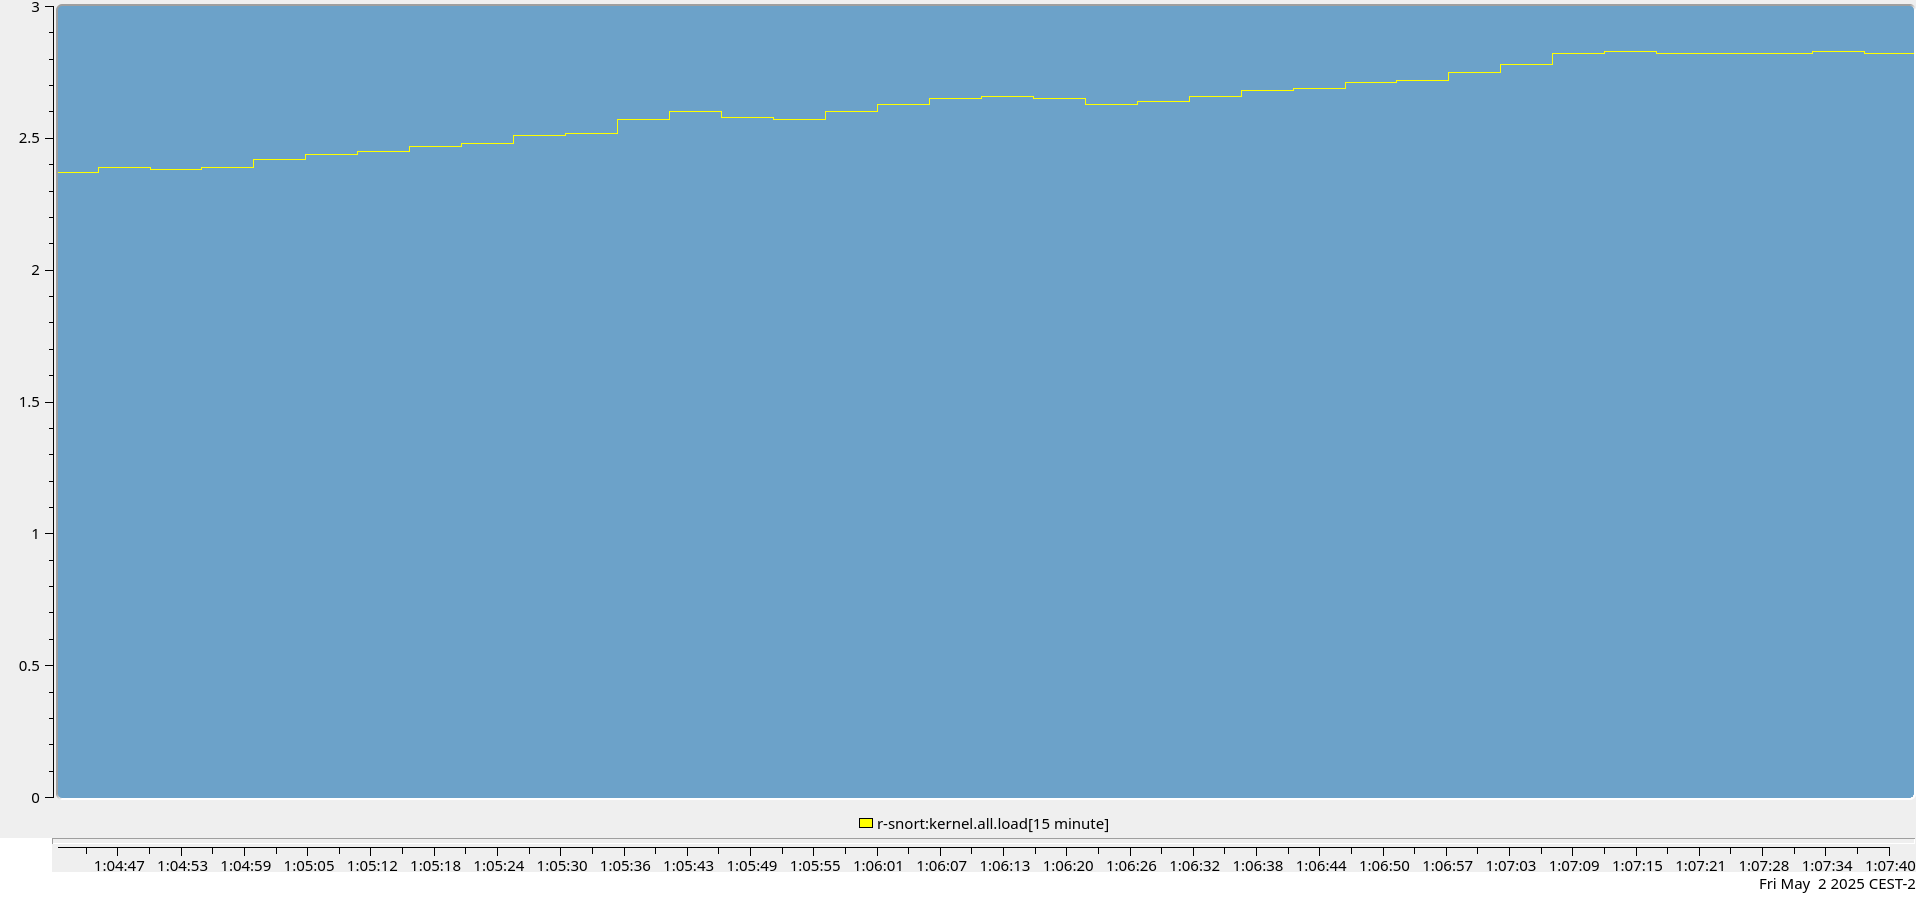
\includegraphics[width=0.9\textwidth]{documento/1.png}
	\caption{Panel de alertas de Suricata en la interfaz web de pfSense.}
	\label{fig:pfsense-alerts}
\end{figure}

\subsection{Interfaz BASE para Snort}
El \emph{Basic Analysis and Security Engine} (BASE) es una de las interfaces web clásicas para la monitorización de Snort. Derivado originalmente del proyecto ACID (Analysis Console for Intrusion Databases), BASE provee un \textbf{frontal web para consultar y analizar las alertas} generadas por un sistema Snort \cite{base}. Este sistema está construido sobre una arquitectura LAMP, empleando un servidor web Apache con páginas PHP que consultan los datos almacenados en una base de datos MySQL. En otras palabras, Snort vuelca sus eventos de alerta en una base de datos y BASE permite explotarlos mediante consultas dinámicas.\newline

A diferencia de pfSense, BASE se centra exclusivamente en el \textbf{análisis de las alertas} y no ofrece funciones para cambiar la configuración del sensor IDS. Su fortaleza radica en las capacidades de 
\textbf{filtrado y agrupación de información} que brinda al analista. La interfaz permite generar consultas predefinidas y personalizadas: por ejemplo, listar las alertas más recientes únicas, obtener las cinco alertas que más se repiten, o visualizar las direcciones IP origen y destino más frecuentes en los registros de intrusiones. La Figura \ref{fig:base-stats} ilustra una de estas visualizaciones, mostrando un resumen de las direcciones IP más detectadas en las alertas. Con estas funciones, BASE facilita identificar patrones de ataque (como hosts atacantes recurrentes o tipos de alertas predominantes) de forma más eficiente que revisando listas planas de eventos.\newline

En términos de \textbf{usabilidad}, la interfaz de BASE, si bien es de corte tradicional, resulta útil para un análisis forense o de seguimiento de incidentes, ya que presenta opciones de búsqueda por múltiples criterios (IP, puerto, fecha, tipo de firma, etc.) y organiza los resultados en formato tabular paginado. No obstante, su diseño es menos interactivo y visual comparado con herramientas modernas: carece de gráficos integrados avanzados o mapas de ataque, y su estética refleja la era en que fue desarrollada (aproximadamente mediados de la década de 2000). Aun así, BASE continúa siendo una referencia en cuanto a funcionalidad de consulta de alertas Snort, proporcionando una base sólida de características sobre la cual se pueden concebir mejoras. Por ejemplo, la idea de incluir filtros por rango temporal o listas de “Top N” alertas en R-Snort toma inspiración directa de este tipo de funcionalidades ya presentes en BASE.

\begin{figure}[hbtp]
	\centering
	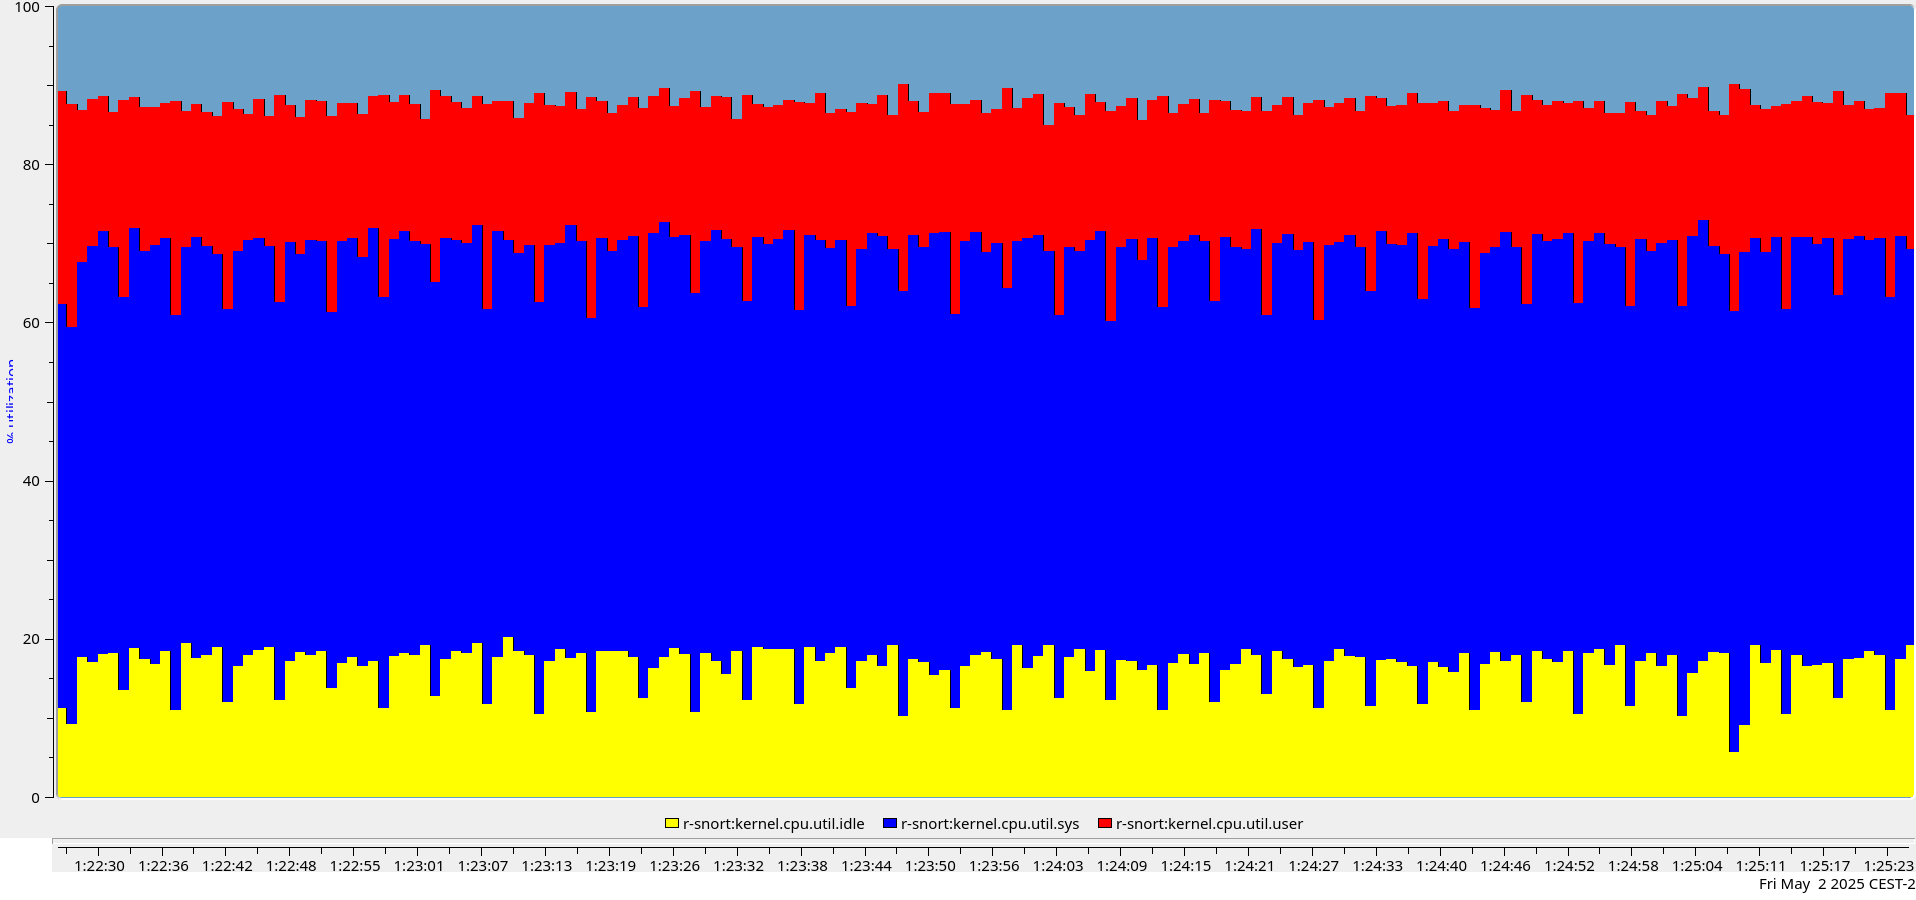
\includegraphics[width=0.85\textwidth]{documento/2.png}
	\caption{Consulta de BASE.}
	\label{fig:base-stats}
\end{figure}

\subsection{Interfaz web de Suricata en T-Pot}
T-Pot es una plataforma integral de \emph{honeypots} mantenida por Telekom Security, que incluye múltiples sensores de seguridad (como Cowrie, Dionaea, conpot, entre otros) y utiliza a Suricata como motor IDS de red. Uno de los atractivos principales de T-Pot es su moderna interfaz de visualización basada en el stack ELK (Elastic Stack). Esta interfaz brinda \textbf{paneles de control gráficos e interactivos} para los datos de alerta. En el caso de Suricata, T-Pot ofrece un panel web integrado (basado en Kibana) que permite analizar las alertas detectadas de forma muy visual. Esta interfaz muestra, por ejemplo, el número total de alertas en un intervalo de tiempo, distribuciones por tipos de amenaza o reglas disparadas, y representaciones como histogramas de eventos en el tiempo y mapas geográficos de las IP de origen de ataques. De hecho, T-Pot soporta "innumerables opciones de visualización" mediante Elastic Stack e incluye mapas de ataque en tiempo real \cite{tpot}. Esto proporciona una experiencia de monitoreo más rica y profesional comparada con las interfaces tradicionales.\newline

Al igual que BASE, la consola de Suricata en T-Pot está enfocada en la \textbf{inspección y análisis} de las alertas, sin exponer opciones para reconfigurar el IDS desde la web. Sin embargo, T-Pot supera a BASE en cuanto a presentación: la disponibilidad de gráficos interactivos y estadísticas automáticas facilita la interpretación rápida del estado de seguridad. Además, la interfaz permite aplicar \textbf{filtros dinámicos} sobre los datos: por ejemplo, es posible filtrar las alertas por una dirección IP específica para ver sólo eventos relacionados con esa fuente, o limitar la vista a un rango temporal definido (por ejemplo, las últimas 24 horas o los últimos 5 días) para focalizar el análisis en determinados periodos de actividad. Estas capacidades de filtrado por campo y tiempo aportan una gran flexibilidad al analista, similar a la que se obtiene con herramientas SIEM, y son implementadas de forma transparente gracias a la potencia de Elasticsearch en el backend.\newline

Desde el punto de vista técnico, la solución de T-Pot es más pesada en recursos que las otras dos interfaces: requiere correr contenedores Docker con Elasticsearch, Logstash y Kibana, entre otros componentes, lo cual demanda memoria y almacenamiento significativos. No obstante, este costo se ve compensado por la \textbf{riqueza funcional} que ofrece en monitorización. En entornos donde se despliega T-Pot, normalmente dedicados a investigación de amenazas o vigilancia de \emph{honeypots}, esta interfaz ha demostrado ser muy efectiva para identificar patrones de ataque complejos y correlaciones entre eventos. La Figura \ref{fig:tpot-dashboard} muestra un ejemplo del panel principal de Suricata en T-Pot, donde se aprecian varias visualizaciones simultáneas de los datos de alerta.\newline

\begin{figure}[hbtp]
	\centering
	\includegraphics[width=0.9\textwidth]{documento/3.png}
	\caption{Panel principal de Suricata en T-Pot.}
	\label{fig:tpot-dashboard}
\end{figure}

\vspace{1em}
\noindent Una comparativa resumida de las funcionalidades de estas interfaces se presenta en la Tabla \ref{tab:comparativa-interfaces}. Puede observarse que cada solución prioriza un aspecto diferente: pfSense destaca en configurabilidad del IDS, BASE en capacidades de consulta detallada, y T-Pot en visualización avanzada. Estas perspectivas complementarias han sido consideradas en el diseño de R-Snort, buscando integrar lo mejor de cada enfoque. En particular, se procura que R-Snort combine la \textbf{gestión configurable} del sensor (inspirada por pfSense) con \textbf{mecanismos de análisis exhaustivo y visualización intuitiva} (tomando como referentes las fortalezas de BASE y T-Pot, respectivamente).

\begin{table}[hbtp]
	\centering
	\renewcommand{\arraystretch}{1.6}
	\setlength{\tabcolsep}{8pt} % Espaciado horizontal entre columnas
	\begin{tabularx}{\textwidth}{|>{\centering\arraybackslash}X 
			|>{\centering\arraybackslash}X 
			|>{\centering\arraybackslash}X 
			|>{\centering\arraybackslash}X|}
		\hline
		\textbf{Característica} & \textbf{BASE (Snort)} & \textbf{pfSense (Suricata)} & \textbf{T-Pot (Suricata)} \\
		\hline
		Configuración del IDS & No & Sí (completa) & No \\
		\hline
		Filtrado de alertas & Sí (varios criterios) & No & Sí (por IP, tiempo, etc.) \\
		\hline
		Visualización gráfica & Limitada (tablas/listas) & No & Sí (gráficos, mapas, \emph{dashboards}) \\
		\hline
		Tecnología backend & LAMP (Apache/PHP/MySQL) & Integrado en GUI (PHP) & Elastic Stack (Kibana/Elasticsearch) \\
		\hline
		Enfoque principal & Análisis forense de alertas & Gestión de IDS/Firewall & \emph{Honeypot} con monitorización \\
		\hline
	\end{tabularx}
	\caption{Comparativa de funcionalidades de las interfaces web de IDS analizadas.}
	\label{tab:comparativa-interfaces}
\end{table}

\clearpage
\null
\thispagestyle{empty}
\newpage
\chapter{Diseño e implantación de un frontend para R-Snort}

\section{Introducción}
En este capítulo se describe el diseño técnico y la implementación de la interfaz web (\emph{frontend}) y la arquitectura general del sistema \textbf{R-Snort}. Este sistema integra el motor de detección de intrusiones Snort en su versión 3 ejecutándose sobre una placa \textbf{Raspberry Pi}, junto con una aplicación web desarrollada en Angular (versión 17) y un servicio backend basado en Spring Boot (Java). El objetivo es convertir la instancia de Snort en un \emph{agente} de seguridad monitorizable de forma remota a través de una interfaz web intuitiva y un conjunto de \emph{dashboards} gráficos para alertas y métricas.\newline

R-Snort adopta una arquitectura modular y desacoplada. Por un lado, la Raspberry Pi actúa como \textbf{sensor IDS} ejecutando Snort 3 y exponiendo una \textbf{API REST} mediante el backend Spring Boot; por otro lado, un cliente web Angular permite al usuario interactuar con el sistema (visualizar alertas, configurar parámetros, etc.). Además, se integra la plataforma \textbf{Grafana} para la visualización en tiempo real de las alertas y métricas de rendimiento a través de paneles personalizados. Todos estos componentes se comunican de forma coordinada para proporcionar una solución unificada de monitorización de intrusiones en la red.\newline

Una de las razones para elegir \textbf{Snort 3} como núcleo del sistema es que esta versión ofrece mejoras significativas en eficiencia y escalabilidad respecto a Snort 2.X, incluyendo una arquitectura \emph{multihilo} capaz de aprovechar sistemas multi-núcleo \cite{snort3differences}. Esto resulta en mayor rendimiento y extensibilidad, aspectos clave al desplegar un IDS en hardware limitado como Raspberry Pi. En efecto, Snort 3.0 presenta un diseño renovado y un superconjunto de funcionalidades de Snort 2, logrando mejor eficacia, rendimiento, escalabilidad, usabilidad y extensibilidad. Gracias a esta capacidad multihilo de Snort 3, es posible utilizar todos los núcleos de la Raspberry Pi 5 para el procesamiento de tráfico, aumentando la tasa de análisis de paquetes.\newline

Para la implementación del backend web, se decidió utilizar el framework \textbf{Spring Boot} por su madurez y las facilidades que ofrece (inicio rápido, servidor web embebido, integración con bibliotecas de seguridad, acceso a bases de datos, etc.). Se consideró incluso una alternativa basada en Python como FastAPI, conocida por su alto rendimiento en servicios REST \cite{FastAPI}, pero finalmente Spring Boot fue elegido por su robustez y por alinear mejor con los conocimientos y requisitos del proyecto (facilidad de integración con Snort a bajo nivel, uso de JDBC para base de datos, etc.) aunque ka herramienta de FastAPI ha servido para la implementación de los agentes individuales. La comunicación entre el frontend Angular y el backend Spring Boot se realiza mediante peticiones HTTP a la API REST, utilizando datos en formato JSON. Para proteger estas comunicaciones y restringir el acceso solo a usuarios autorizados, el sistema implementa autenticación basada en \textbf{JSON Web Tokens (JWT)}. Un JWT es un estándar abierto (RFC 7519) que define un método compacto y seguro de transmitir información entre partes en formato JSON \cite{JWT}, lo que permite verificar la identidad del usuario sin mantener sesiones en el servidor. De este modo, el frontend obtiene un token JWT tras el inicio de sesión y lo incluye en las cabeceras de las peticiones subsecuentes, garantizando un acceso seguro a las funcionalidades de R-Snort.\newline

En la Figura \ref{fig:arquitectura} se muestra un diagrama general de la arquitectura de R-Snort. En dicha ilustración se aprecian los principales componentes: la Raspberry Pi ejecuta Snort 3 como agente sensor junto al servicio backend (API REST) que interactúa con Snort y con la base de datos de alertas, el servicio de FAST API; el usuario accede desde un navegador web al frontend Angular, el cual consume la API para presentar información y opciones de configuración; finalmente, Grafana se conecta a la fuente de datos de alertas (base de datos) para ofrecer paneles gráficos actualizables en tiempo real.\newline

\begin{figure}[hbtp]
	\centering
	 \includegraphics[width=0.8\textwidth]{documento/5.png}
	\caption{Arquitectura general del sistema R-Snort.}
	\label{fig:arquitectura}
\end{figure}

En las secciones siguientes se detallan, primero, las especificaciones y requisitos del sistema (funcionales y técnicos) y, a continuación, el entorno de trabajo utilizado, tanto a nivel de hardware (la plataforma Raspberry Pi empleada como agente de seguridad) como de software (componentes instalados, configuraciones relevantes y herramientas auxiliares). Asimismo, se describe brevemente el entorno de desarrollo y pruebas, donde se aclaran las tecnologías usadas para implementar el frontend y backend, así como la configuración de la red de laboratorio empleada para validar el funcionamiento de R-Snort.\newline

\section{Especificaciones del sistema}
A continuación, se enumeran las principales \textbf{características y requisitos} que se definieron para el sistema R-Snort, abarcando tanto funcionalidades esperadas como consideraciones de diseño e implantación:\newline

\begin{itemize}
	\item \textbf{Motor IDS basado en Snort 3:} El sistema debe emplear Snort en su versión 3 como núcleo de detección de intrusiones. Snort 3 proporciona capacidades mejoradas (p. ej., soporte multihilo, nuevos plugins y sintaxis de reglas mejorada) que incrementan la eficacia y rendimiento de la detección.
	
	\item \textbf{Plataforma hardware accesible:} El IDS ha de poder ejecutarse sobre una Raspberry Pi, aprovechando la portabilidad y bajo coste de este dispositivo. Esto permite desplegar el sensor en entornos domésticos o de pequeña empresa sin requerir hardware dedicado costoso.
	
	\item \textbf{Interfaz web para gestión y monitoreo:} Se requiere un frontend amigable, accesible vía navegador, que permita al usuario administrar el sistema y visualizar las alertas detectadas. Este frontend se desarrollará como una \emph{Single Page Application} en Angular, garantizando una experiencia interactiva y fluida.
	
	\item \textbf{Backend RESTful:} La arquitectura debe seguir un modelo cliente-servidor desacoplado. Para ello, se implementará una API REST en el backend (usando Spring Boot y FAST API) que exponga las funcionalidades necesarias: consulta de alertas, estado de Snort, gestión de configuración, etc. Este backend actúa de intermediario entre Snort, la base de datos y el frontend.
	
	\item \textbf{Visualización de alertas y métricas:} El sistema debe ser capaz de presentar no solo listados de alertas, sino también gráficos y métricas agregadas. Se integrará \textbf{Grafana} para este propósito, configurando \emph{dashboards} que muestren por ejemplo el número de alertas por tipo, tendencias temporales, y métricas de rendimiento (CPU, uso del disco, etc.). Grafana es una plataforma de monitorización y visualización de datos de código abierto ampliamente utilizada en la industria para analítica interactiva \cite{Grafana}.
	
	\item \textbf{Almacenamiento persistente de datos:} Las alertas de intrusión y otros datos relevantes deben almacenarse en una base de datos para permitir su consulta histórica y correlación. Se optó por utilizar una base de datos relacional \textbf{MariaDB} (derivada de MySQL) como repositorio principal de alertas.
	
	\item \textbf{Gestión de reglas y configuración de Snort:} La solución debe facilitar la administración de Snort sin requerir acceder directamente por consola. Esto incluye la posibilidad de agregar reglas IDS (por ejemplo, descargar nuevas reglas de la comunidad o de Snort), eliminar conjuntos de reglas según las necesidades, y ajustar parámetros de configuración de interfaces a través de la web o la API.
	
	\item \textbf{Seguridad y control de acceso:} Dado que la interfaz de gestión expone funcionalidades críticas (ej. ver alertas de seguridad, modificar reglas), es imprescindible restringir el acceso solo a usuarios autorizados. Para ello, se integra un mecanismo de autenticación basado en JWT tal como se mencionó, de forma que cada administrador de R-Snort deba iniciar sesión para obtener un token válido. La comunicación entre frontend y backend debe estar protegida (idealmente usando HTTPS para entornos de producción, evitando la transmisión de credenciales o tokens en texto claro).
	
	\item \textbf{Registro y rotación de \emph{logs}:} Snort genera archivos de registro de alertas que pueden crecer rápidamente. El sistema debe implementar esquemas de \emph{log rotation} para controlar el tamaño de los logs y evitar agotar el espacio en la Raspberry Pi. Por ejemplo, mediante herramientas del sistema (como \texttt{logrotate} en Linux) se rotarán y comprimirán periódicamente los archivos de alertas, manteniendo un histórico reciente y eliminando registros antiguos de forma automatizada.
	
	\item \textbf{Scripts de instalación automatizada:} Para facilitar la puesta en marcha del sistema, se prepararon \emph{scripts} modulares que automatizan la instalación y configuración de los distintos componentes (Snort 3, base de datos MariaDB, entorno Grafana, despliegue del backend Spring Boot, etc.). Cada módulo de instalación puede ejecutarse independientemente, permitiendo por ejemplo instalar solo el agente Snort en una máquina o solo el servidor web en otra, según la arquitectura deseada. Esto refleja la filosofía modular de R-Snort, haciendo posible su adaptación o escalado a futuros despliegues (por ejemplo, múltiples sensores Snort en distintas Raspberry Pi reportando a un servidor central).
	
	\item \textbf{Rendimiento aceptable en hardware limitado:} Se exige que el sistema funcione de manera estable en la Raspberry Pi, atendiendo a sus limitaciones de CPU, memoria y E/S. Esto implica optimizar la configuración de Snort (por ejemplo, cargar únicamente las reglas necesarias, ajustar hilos de procesamiento) y minimizar el consumo de recursos del backend y la base de datos. Las pruebas deben verificar que el IDS puede manejar el tráfico de la red objetivo (típicamente redes domésticas o de oficina pequeña) sin pérdidas de paquetes significativas y con latencia aceptable en la interfaz web.
\end{itemize}

En síntesis, los requisitos anteriores delinean un sistema completo de detección de intrusos gestionable vía web, construido con tecnologías modernas y enfocado en facilidad de uso, todo ello sobre una plataforma de bajo coste. A continuación, se detalla el entorno de trabajo y la arquitectura de los componentes que dan cumplimiento a estas especificaciones.\newline

\section{Entorno de trabajo}
En esta sección se describe el entorno de hardware y software utilizado para implementar R-Snort, así como el entorno de desarrollo y pruebas empleado durante la construcción del sistema. Se hace énfasis en la configuración de la Raspberry Pi como agente de seguridad, en los componentes de software integrados (Snort 3, complementos y herramientas auxiliares), y en cómo se llevó a cabo el desarrollo del frontend y backend y su validación en un entorno controlado.\newline

\subsection{Hardware: Raspberry Pi como agente de seguridad}
El dispositivo hardware central de la solución es una \textbf{Raspberry Pi}, empleada aquí como un agente de seguridad en la red. En concreto, se utilizó una Raspberry Pi 5, que cuenta con un procesador Quad-core Arm Cortex-A76 a 2,4 GHz y 8 GB LPDDR4X de memoria RAM, capacidades suficientes para ejecutar un IDS ligero junto con un servidor web básico. La Raspberry Pi se eligió por varias razones: es un equipo de bajo coste y tamaño reducido, con un consumo eléctrico mínimo, lo que permite tener un sensor de red siempre activo sin apenas impacto económico; además, su tamaño compacto facilita ubicarla directamente en el entorno de red a monitorizar (por ejemplo, junto al router o switch principal de la organización).\newline

A pesar de sus recursos limitados, la Raspberry Pi ha demostrado ser capaz de albergar sistemas IDS/IPS funcionales en escenarios de pequeña escala. Por ejemplo, existen guías prácticas que muestran cómo convertir una Raspberry Pi en un IDS/IPS completamente funcional capaz de detectar intrusiones en la red. De hecho, la comunidad de seguridad ha validado la viabilidad de esta aproximación, aprovechando la portabilidad y suficiencia de procesamiento que ofrece este microordenador \cite{SecMaster2024}. En nuestro caso, la Pi actúa como un \emph{appliance} de seguridad dedicado: captura el tráfico de la red, ejecuta Snort para analizar dicho tráfico en busca de patrones maliciosos, y envía las alertas generadas a los subsistemas correspondientes (base de datos, interfaz web, dashboards, etc.).\newline

La forma de \textbf{integración en la red} de la Raspberry Pi depende del modo de funcionamiento del IDS. En este proyecto, R-Snort se despliega en modo \emph{pasivo} (IDS puro, no IPS), es decir, la Pi monitoriza el tráfico sin interrumpirlo. Para lograr esto, una práctica común es conectar la interfaz de red de la Pi a un puerto espejo (\emph{mirror/span port}) de un switch, o en su defecto, colocarla en la misma subred que los equipos a vigilar y configurar reglas apropiadas de captura. De esta manera, la Pi recibe copias del tráfico de red pero no introduce latencia ni punto de falla en la comunicación. Alternativamente, si se buscara un modo \emph{inline} (IPS), sería necesario contar con dos interfaces de red en la Raspberry Pi y configurarla como puente; sin embargo, para simplificar la implantación, R-Snort se centra en la monitorización pasiva.\newline

En la Figura \ref{fig:despliegue} se ilustra un posible \textbf{esquema de despliegue} de R-Snort en una red local. La Raspberry Pi está conectada al switch de la red mediante cable Ethernet; el switch está configurado para duplicar el tráfico de los dispositivos hacia el puerto donde se encuentra la Pi, permitiendo que Snort inspeccione los paquetes. El administrador puede acceder al frontend web y a los paneles de Grafana desde un equipo en la misma red (o remotamente vía VPN), conectándose a la dirección IP de la Raspberry Pi. Así, la Pi actúa como nodo de monitoreo, analizando el tráfico y reportando alertas sin interferir en la comunicación normal de la red.\newline

\begin{figure}[hbtp]
	\centering
	\includegraphics[width=0.8\textwidth]{documento/4.png}
	\caption{Esquema de despliegue de R-Snort en la red local.}
	\label{fig:despliegue}
\end{figure}

En cuanto al \textbf{sistema operativo} utilizado en la Raspberry Pi, se optó por una distribución Linux de 64 bits para garantizar compatibilidad con Snort 3 y un buen aprovechamiento de la memoria. En particular, se empleó Ubuntu Server de 64 bits. Esta elección minimiza la carga de procesos innecesarios y permite dedicar la mayor parte de los recursos al IDS y al servidor web. Todas las interacciones con la Pi (instalación de paquetes, edición de configuraciones, revisión de logs) se realizaron vía acceso remoto SSH, ya que la Pi operaba en modo head-less (sin monitor ni periféricos).\newline

Es importante resaltar que, aunque la Raspberry Pi 5 ofrece un rendimiento notable para su tamaño, sigue estando lejos de un hardware de servidor. Por ello, el volumen de tráfico que puede analizar en tiempo real es limitado. En entornos de alta carga (por ejemplo, redes gigabit con tráfico sostenido muy elevado) es posible que la Pi se vea sobrepasada. Sin embargo, para entornos objetivo de este proyecto (redes domésticas o PYMEs, típicamente con anchos de banda de decenas de Mbps y tráfico intermitente), la capacidad de la Pi es adecuada. Estudios de rendimiento han mostrado que Snort (y herramientas similares como Suricata) corriendo en una Raspberry Pi pueden llegar a inspeccionar del orden de cientos de Mb/s con configuraciones optimizadas \cite{SecMaster2024}, lo cual cubre las necesidades planteadas. En cualquier caso, durante las pruebas se ha monitorizado el uso de CPU, memoria y red de la Pi para asegurar que el sistema operaba dentro de márgenes seguros.\newline

\subsection{Software: Snort 3 y complementos}
A nivel de software, el componente principal es el \textbf{motor IDS Snort 3}. Snort es un sistema de detección de intrusiones de código abierto ampliamente utilizado, basado en análisis de firmas/patrones definidos en reglas. La versión 3 de Snort representa una reimplementación moderna del IDS clásico, aportando una serie de mejoras que resultan beneficiosas para este proyecto. Entre ellas cabe mencionar el soporte multi-hilo (permitiendo procesar paquetes en paralelo), un nuevo lenguaje de reglas más flexible, y la disponibilidad de más de 200 complementos o \emph{plugins} para diversas funcionalidades. Todas estas mejoras conllevan una mayor eficiencia y facilidad de extensión del IDS, factores cruciales al desplegarlo en un entorno limitado pero que puede requerir personalizaciones.\newline

En R-Snort, Snort 3 se configuró en \textbf{modo IDS} (no bloquea tráfico, solo alerta) y se ejecuta como servicio en la Raspberry Pi. Se personalizó el archivo de configuración de Snort (en formato Lua, propio de Snort3) para adaptarlo a la red local monitorizada: se definió la variable \texttt{HOME\_NET} con el rango de IP interno a proteger, se ajustaron los puertos considerados para ciertos protocolos (por ejemplo incluir puertos de servicios comunes en la red local) y se activaron preprocesadores relevantes (como \emph{Stream5} para seguimiento de sesiones TCP, \emph{HTTP Inspect} para analizar tráfico web, etc.). Asimismo, se habilitó la salida de alertas en \textbf{formato JSON}, mediante el uso del \emph{plugin} \texttt{alert\_json}, de modo que cada evento de alerta que genera Snort se registra como una entrada JSON estructurada (conteniendo campos como timestamp, dirección IP de origen y destino, puerto, identificación de la regla que se disparó, mensaje de alerta, etc.). Este formato resulta conveniente para su posterior procesamiento automatizado por otras partes del sistema.\newline

Adicionalmente, se utilizaron ciertos \textbf{complementos de Snort} necesarios para su correcto funcionamiento en Raspberry Pi. En particular, se instaló la librería \textbf{DAQ} (\emph{Data Acquisition}) apropiada para capturar el tráfico de red; en este caso, se usó \texttt{af\_packet} (incluida con Snort 3) que permite leer directamente de la interfaz de red en modo promiscuo con buen rendimiento. También se configuró Snort para que se ejecute con privilegios limitados por seguridad (utilizando el usuario \texttt{snort} y grupo \texttt{snort} creados en el sistema) y se creó un servicio \texttt{systemd} para su lanzamiento automático en el arranque de la Pi.\newline

Otro aspecto importante es la gestión de las \textbf{reglas IDS}. Para este proyecto, se decidió comenzar utilizando las \emph{reglas comunitarias} gratuitas de Snort (Snort Community Rules) y algunas reglas emergentes de Emerging Threats, para disponer de un conjunto base que cubra amenazas comunes. Se implementó un script de actualización que, bajo demanda o de forma programada, descarga las últimas reglas (mediante \emph{oinkcode} si aplica, en el caso de Snort) y actualiza el directorio de reglas de Snort. Así, desde la interfaz de R-Snort, el usuario podría desencadenar la actualización de reglas sin tener que hacerlo manualmente. Aunque herramientas clásicas como \texttt{PulledPork} aún no tienen versión oficial para Snort 3, se logró una funcionalidad similar mediante scripts en Bash que automatizan la descarga y colocación de nuevos archivos de reglas, seguidos de un reinicio suave de Snort para aplicar los cambios. (Ver el complemento de TFG para más detalles).\newline

Además del propio Snort, el sistema incorpora varios \textbf{componentes software complementarios} que, en conjunto, constituyen la solución completa:\newline

\textbf{Backend central en Spring Boot:}
Desarrollado en Java 17 mediante el framework Spring Boot, este módulo no se instala en las Raspberry Pi (agentes), sino que reside en el servidor principal, actuando como centro de control y despliegue del sistema. Su función se limita a gestionar la autenticación, la gestión de usuarios y la coordinación de los distintos agentes de la red. Para ello, expone varios endpoints REST como \texttt{/api/login} (para iniciar sesión mediante credenciales y obtener un token JWT), \texttt{/api/agents} (para listar y registrar agentes disponibles). Un \textbf{agente} en este contexto es una Raspberry Pi con Snort y el software auxiliar instalado, dedicada a monitorizar el tráfico de red local de una ubicación concreta. Cada agente se comunica con el backend central para facilitar la administración remota y permitir que un único punto de control visualice, gestione y configure todos los nodos desplegados.\newline

\textbf{Backend local en cada agente (FastAPI):}
Cada Raspberry Pi funciona de manera autónoma como agente de monitorización, gracias a un backend ligero desarrollado en Python mediante FastAPI, denominado internamente \texttt{fasatpi}. Este componente se instala localmente en cada dispositivo o módulo de R-Snort y es el encargado de proporcionar la información propia del agente a la interfaz web. Expone endpoints REST como \texttt{/alerts}, \texttt{/status}, \texttt{/rules} o \texttt{/logs}, los cuales permiten consultar alertas generadas, comprobar el estado de Snort, gestionar reglas o descargar logs archivados.
Internamente, \texttt{fasatpi} accede a los archivos JSON generados por Snort, así como a la base de datos local MariaDB donde se almacenan las alertas y métricas. Además, implementa acciones sobre el sistema, como reiniciar Snort mediante scripts o comprobar el estado de servicios mediante comandos shell. Gracias a este diseño, cada agente puede funcionar de forma autónoma incluso sin conexión constante al backend central, y ofrece una interfaz clara para que R-Snort WebApp pueda consultar y controlar su estado desde la red.\newline

\textbf{Base de datos MariaDB:} Para persistir las alertas y otros datos, se configuró un servidor de base de datos MariaDB 10.x corriendo en la propia Raspberry Pi. Cada alerta generada por Snort es insertada en una tabla (p. ej. \texttt{alerts}) con campos como timestamp, IP origen, IP destino, puerto, protocolo, SID de la regla, mensaje, etc. Esta inserción se realiza de manera automática: el backend Spring Boot incluye un componente que supervisa la aparición de nuevas entradas en el log JSON de Snort (mediante un hilo que observa el archivo o utilizando mecanismos de notificación del sistema de ficheros) y en cuanto detecta una nueva alerta, la parsea del JSON e inserta los datos en la base MariaDB mediante JDBC. De esta forma, construimos una \textbf{pipelines} de datos desde Snort hacia la base de datos casi en tiempo real. Cabe mencionar que Grafana y el propio frontend consultarán esta base para mostrar la información al usuario.\newline

\textbf{Grafana:} Es la herramienta seleccionada para la visualización gráfica de los datos. Grafana es una aplicación web de monitoreo que permite crear paneles interactivos a partir de diversas fuentes de datos (tiempo real, series temporales, etc.) \cite{Grafana}. En R-Snort, se instaló Grafana OSS (código abierto) versión 12 en la Raspberry Pi, aprovechando que existen builds para arquitectura ARM. La instancia de Grafana se configuró para conectarse a la base de datos MariaDB como \emph{data source} utilizando el conector MySQL. De esta forma, se pudieron escribir consultas SQL sobre la tabla de alertas y representar resultados en gráficas. Grafana se ejecuta como un servicio aparte, corriendo en el puerto 3000 de la Raspberry Pi, y la interfaz Angular tiene la opción de embeber ciertos paneles de Grafana mediante iframes o bien el usuario puede acceder directamente al dashboard completo de Grafana para análisis más avanzados. Ambos (frontend propio y Grafana) beben de la misma base de datos de alertas, garantizando consistencia en la información.\newline

\textbf{Rotación de logs y mantenimiento:} A nivel de sistema operativo, se añadieron configuraciones para mantener el sistema funcionando sin intervención manual. En particular, se creó una tarea \texttt{cron} diaria que ejecuta \texttt{logrotate} sobre los archivos de log de Snort (y opcionalmente logs del backend), de modo que cada día se archiva el log del día anterior y se comienza uno nuevo, conservando, por ejemplo, solo 7 días de logs comprimidos. Asimismo, se desarrollaron pequeños scripts de \emph{health-check} que comprueban si el proceso de Snort sigue activo y, si no, intentan reiniciarlo usando \texttt{systemctl}; esto agrega robustez frente a eventuales caídas del IDS. El backend Spring Boot se configuró también como servicio de sistema para iniciarse automáticamente en el arranque (\texttt{systemd service}) y reiniciarse en caso de falla.\newline

En resumen, la Raspberry Pi ejecuta de forma concurrente varios servicios: Snort 3 (detección de intrusos), Spring Boot (API REST y lógica de negocio), FAST API (datos del sistema), MariaDB (almacenamiento de datos) y Grafana (visualización). Gracias a la optimización y a la moderada carga esperada, la Pi es capaz de manejar estos componentes simultáneamente. Cada uno cumple un rol específico pero se complementan para brindar la funcionalidad global de R-Snort. El diseño modular permite incluso que, de ser necesario, alguno de estos componentes pudiera desplazarse a otro equipo (por ejemplo, usar un servidor externo para Grafana o la base de datos) sin grandes cambios, evidenciando la flexibilidad de la arquitectura planteada.\newline

\subsection{Entorno de desarrollo}
El desarrollo del frontend y backend de R-Snort se llevó a cabo utilizando herramientas modernas y siguiendo buenas prácticas para garantizar la calidad del software. Para la parte de \textbf{frontend Angular}, se empleó \textbf{TypeScript} como lenguaje de programación y el \emph{framework} Angular en su versión 19. La estructura del proyecto Angular se inicializó con \texttt{angular-cli}, organizando los componentes, servicios y rutas de la aplicación de forma modular. Durante la implementación, se hizo uso de un conjunto de librerías de interfaz comunes (por ejemplo, Angular Material) para agilizar la construcción de elementos UI como tablas, diálogos modales y gráficos simples. El entorno de desarrollo incluyó herramientas como \textbf{Visual Studio Code} como editor principal y el servidor de desarrollo de Angular (\texttt{ng serve}) que permitía ver los cambios en vivo en el navegador durante la codificación. Para el manejo de versiones del código se utilizó Git, lo cual facilitó llevar un control de cambios y colaborar en caso de integración de diferentes partes.\newline

En cuanto al \textbf{backend Spring Boot}, se utilizó el \emph{stack} típico de Spring: Spring MVC para la creación de controladores REST, Spring Data JPA para la capa de persistencia con MariaDB (definiendo entidades JPA que representan las alertas, etc.), y Spring Security para implementar la capa de autenticación JWT. El proyecto se configuró con \texttt{Maven} como gestor de dependencias. Durante el desarrollo, se probaban los endpoints localmente en un equipo de escritorio antes de desplegarlos en la Raspberry Pi, usando herramientas como \textbf{Postman} para verificar las respuestas JSON de la API. Una vez validados, el backend se compilaba en un \emph{JAR ejecutable} (\texttt{spring-boot fat jar}) y se transfería a la Pi para su ejecución en producción. La Pi cuenta con OpenJDK 17 instalado para correr la aplicación Java.\newline

Para asegurar la \textbf{integración del frontend con el backend}, se habilitó \textbf{CORS} (Cross-Origin Resource Sharing), ya que durante la etapa de desarrollo el frontend Angular se ejecutaba en \texttt{localhost:4200} y necesitaba consumir la API alojada en la Raspberry Pi. Spring Boot se configuró para permitir el origen del frontend en desarrollo. En la versión final, al compilar la aplicación Angular para producción, los archivos estáticos (HTML/JS/CSS) del frontend se sirvieron directamente desde el backend (Spring Boot puede servir contenido estático), evitando así problemas de CORS en el uso real.\newline

El entorno de desarrollo se aseguró que todos los componentes de R-Snort funcionaran de manera armónica. La elección de Angular y Spring Boot simplificó la construcción del frontend manteniendo un código mantenible.

\section{Diseño / Arquitectura / Elementos}

\subsection{Diseño de la arquitectura}

El sistema \textbf{R-Snort} presenta una arquitectura distribuida y modular, compuesta por múltiples \emph{agentes} desplegados junto a instancias de Snort y un módulo central que coordina el funcionamiento general.\newline
Cada \texttt{snort-agent} es un componente ligero (desarrollado en Python) que se instala en los equipos a monitorizar junto al software Snort. La instalación del agente es sencilla y automatizada, mediante un script o paquete que despliega Snort, el propio agente y todas sus dependencias (incluyendo la base de datos local MariaDB) sin necesidad de configurar manualmente cada detalle. Una vez instalado, el agente arranca varios servicios internos que gestionan la detección de intrusiones de forma autónoma:\newline
\begin{itemize}
	\item \texttt{ingest\_service.py}: servicio responsable de leer las alertas generadas por Snort (por ejemplo, a través de archivos de log o sockets de Snort) e insertarlas en la base de datos MariaDB local del agente (tabla de alertas).
	\item \texttt{metrics\_timer.py}: proceso en segundo plano que periódicamente recoge métricas del sistema anfitrión (uso de CPU, uso de disco, temperatura de la CPU, etc.) y las almacena en la base de datos local (tabla de métricas del sistema). Esto permite tener un registro histórico del rendimiento y estado de cada sensor.
	\item \texttt{agent\_api.py}: servidor web ligero (implementado con \textit{FastAPI}) que expone una API REST para interactuar con el agente. Este componente proporciona endpoints para consultar el estado (\texttt{/status}) del sensor y de Snort, obtener listas de alertas (\texttt{/alerts}) y métricas (\texttt{/metrics}), gestionar las reglas de detección (\texttt{GET /rules} para listar reglas personalizadas, \texttt{POST /rules} para agregarlas, \texttt{DELETE /rules/{sid}} para eliminarlas) y controlar servicios (\texttt{/services/status} y \texttt{/services/restart} para verificar o reiniciar Snort, entre otros). La API actúa de intermediario entre el nodo sensor y el resto del sistema, permitiendo que el módulo central u otros clientes recuperen datos y emitan órdenes de forma estandarizada.
\end{itemize}

Los \texttt{snort-agent} automatizan gran parte de la configuración y mantenimiento del sistema en cada nodo. Por ejemplo, se encargan de aplicar la configuración de Snort para recoger las alertas en un deterinado fichero y ajustan componentes complementarios del entorno. Incluyen mecanismos para respaldo de datos copias de seguridad periódicas de logs y gestionan la rotación de estos (\emph{logrotate}) para evitar el crecimiento indefinido de los archivos de alertas. Todo ello reduce la intervención manual y facilita un enfoque \emph{plug-and-play}, donde un usuario no técnico puede desplegar un sensor Snort con mínima complejidad.\newline
El \textbf{módulo central} del sistema actúa a la vez como un agente y como el nodo coordinador que concentra la interfaz de usuario y la lógica de negocio. En el servidor central se ejecuta también un \textit{snort-agent} (monitorizando el propio equipo central como un sensor más), pero adicionalmente aloja un backend desarrollado en Spring Boot y el frontend web en Angular. El backend Spring Boot expone una API REST segura (con autenticación JWT) que orquesta la comunicación entre el frontend y los distintos agentes distribuidos. A través de esta capa central, los usuarios pueden autenticarse y realizar consultas unificadas: por ejemplo, solicitar las alertas de un cierto agente, agregar una nueva regla de detección o verificar el estado de todos los sensores. El backend traduce esas solicitudes en llamadas a la API REST de los agentes correspondientes. De este modo, si el usuario solicita datos de un agente remoto, el servidor central invoca el endpoint apropiado del \texttt{agent\_api.py} en ese nodo (por ejemplo \texttt{/alerts} para obtener las alertas recientes desde la base de datos local del agente). Del mismo modo, cuando el usuario emite una acción (p. ej. reiniciar Snort en un sensor), el backend central envía la orden mediante \texttt{/services/restart} al agente seleccionado. Toda la transferencia de datos se realiza en formato JSON sobre HTTP(S), manteniendo un bajo acoplamiento entre módulos y permitiendo escalar o reemplazar componentes fácilmente.\newline
En la Figura \ref{fig:arquitectura} se muestra un esquema general de la arquitectura de R-Snort, donde se aprecian sus elementos principales y las interacciones entre ellos: el usuario accede mediante un navegador al frontend Angular (alojado en el servidor central), el cual se comunica con el backend Spring Boot. El backend a su vez envía peticiones REST hacia los \texttt{snort-agent} distribuidos (incluido el agente del propio servidor central) para recopilar información o ejecutar comandos. Esta arquitectura distribuida y modular permite monitorizar múltiples puntos de la red de forma centralizada y coherente.

\begin{figure}[h!]
	\centering
	\begin{verbatim}
		Usuario (Navegador Web)
		|
		v HTTP/HTTPS (JWT)
		Frontend Angular SPA (Servidor Central)
		|
		v Peticiones REST (JSON)
		Backend Spring Boot (Servidor Central)
		|
		-----------------------------------------------------
		| | |
		Agente Central Agente 1 (Remoto) ... Agente N (Remoto)
		(FastAPI + Snort + DB) (FastAPI + Snort + DB) (FastAPI + Snort + DB)
	\end{verbatim}
	\caption{Esquema de la arquitectura distribuida de R-Snort, mostrando la interacción entre el usuario, el servidor central (backend + frontend) y los agentes Snort remotos.}
	\label{fig:arquitectura}
\end{figure}

En resumen, el diseño plug-and-play de R-Snort está orientado a usuarios no técnicos: agregar un nuevo sensor es tan simple como instalar un agente en el nuevo equipo e informarlo al sistema central, sin configuraciones manuales complejas. Esta aproximación aporta un gran valor en entornos de ciberseguridad distribuida, ya que ofrece visibilidad unificada de múltiples sensores de intrusión. Cada agente opera de manera autónoma en su segmento de red, pero todos son gestionados centralmente, lo que aumenta la cobertura de detección y la resiliencia (si un sensor falla o es comprometido, los demás continúan operativos y reportando al panel central).

\subsection{Diseño de la interfaz de usuario}

El sistema cuenta con una interfaz web de usuario desarrollada en Angular, construida como una \emph{Single Page Application} (\textbf{SPA}) independiente que se comunica con el backend mediante peticiones HTTP a la API REST central. Esta aplicación frontend, desplegada en el servidor central, ofrece una experiencia interactiva y dinámica, con un diseño visual enfocado en el dominio de la ciberseguridad. La usabilidad se ha cuidado para que la información compleja de las alertas y métricas se presente de forma accesible y atractiva incluso para operadores no especializados.\newline
La interfaz de usuario se estructura en varios módulos o pantallas principales, accesibles desde una barra de navegación superior:\newline
\begin{itemize}
	\item \textbf{Inicio de sesión:} es la pantalla inicial de la aplicación, donde el usuario introduce sus credenciales (\emph{correo electrónico} y \emph{contraseña}) para acceder. Tras hacer clic en "Acceder", el backend valida las credenciales y, de ser correctas, emite un token de autenticación JWT. La apariencia de esta vista es sencilla y centrada (formulario sobre fondo oscuro, como se aprecia en la Figura 2.4.2), siguiendo las pautas de diseño minimalista.
	
	\item \textbf{Selector de agente:} una vez autenticado, el usuario puede seleccionar cuál de los agentes disponibles desea monitorizar. En la barra superior de la SPA se muestra un menú desplegable que lista los agentes registrados (identificados por nombre o dirección IP, e.g. "Central (192.168.1.169)"). Al elegir un agente, el frontend carga los datos correspondientes a ese sensor en las vistas de alertas, reglas y estado. Este mecanismo permite controlar múltiples sensores desde la misma interfaz de forma conveniente.
	
	\item \textbf{Vista de alertas:} es el panel principal de monitorización, donde se presentan las detecciones de intrusiones reportadas por Snort en el agente seleccionado. Incluye indicadores numéricos de alertas por nivel de severidad (ej. cantidad de alertas altas, medias, bajas) y una tabla que enumera las últimas alertas detalladas con sus campos clave (hora, descripción de la alerta, IP de origen, IP de destino, puerto implicado, clasificación de la alerta y nivel de severidad). Esta vista permite al analista ver rápidamente qué incidentes se han detectado y su naturaleza. Además, proporciona botones para exportar los datos de alertas en formato CSV: por ejemplo, "Descargar alertas de este agente" genera un archivo con todas las alertas actuales del sensor activo, mientras que "Descargar todas las alertas" consolida las alertas de todos los agentes en un solo fichero (facilitando un análisis global). En la Figura 2.4.3 se ilustra un ejemplo de esta pantalla, mostrando el \emph{Panel de Alertas} con los contadores de severidad y la tabla de alertas recientes.
	
	\item \textbf{Vista de reglas:} sección de la aplicación dedicada a la gestión de reglas personalizadas de Snort en el agente seleccionado. Permite al usuario con rol adecuado agregar nuevas reglas de detección escribiendo la definición en formato Snort en un campo de texto y pulsando "Agregar regla". Una vez enviada, la regla se almacena a través del backend en el agente correspondiente (el \texttt{snort-agent} la añade a la configuración de Snort y recarga el motor de detección para que la nueva regla entre en vigor). Asimismo, en esta vista se listan todas las reglas personalizadas previamente añadidas al sensor, mostrando por cada una su \texttt{SID} (identificador único), el mensaje descriptivo (\texttt{MSG}) y la sintaxis completa de la regla. Junto a cada regla se presenta una opción (icono de papelera) para eliminarla si es necesario, lo cual provoca que el agente la remueva de Snort (actualizando la configuración). La Figura 2.4.4 muestra la interfaz de esta vista de reglas, donde se observan el formulario de nueva regla y la lista de reglas existentes con sus detalles.
	
	\item \textbf{Vista de estado del sistema:} pantalla orientada a visualizar las métricas operativas del agente y el estado del servicio Snort. Contiene gráficas en tiempo real de los datos del sistema recabados (por ejemplo, un gráfico de línea de la temperatura de CPU del sensor, y otro del porcentaje de uso de CPU y de disco a lo largo del tiempo). Estos gráficos ofrecen al usuario una idea del rendimiento y condiciones del hardware donde corre Snort, ayudando a detectar posibles sobrecargas o problemas (p.ej., temperatura anómala). Además, esta vista muestra el estado actual de Snort en ese agente: indica si el proceso IDS está \emph{Activo} y la marca de tiempo de la última alerta registrada. Si el usuario cuenta con permisos de administrador, desde aquí puede reiniciar remotamente el servicio Snort en el agente seleccionado mediante un botón dedicado ("Reiniciar Snort"). También se listan en esta página los \emph{logs} archivados (ficheros históricos de alertas comprimidos tras la rotación de logs); el usuario puede descargarlos para un análisis forense si es necesario. En la Figura 2.4.5 se aprecia esta sección, incluyendo un ejemplo de gráfico de temperatura CPU y los indicadores de estado del agente.
	
	\item \textbf{Overview e integración con Grafana:} la página inicial del panel (denominada \emph{Overview}) ofrece un resumen gráfico consolidado de la información de seguridad. Esta vista integra paneles de visualización tipo \emph{dashboard} para representar las alertas y eventos de forma gráfica y amigable, aprovechando herramientas como Grafana para las métricas de serie temporal. Por ejemplo, se muestran diagramas de dona con la distribución de alertas por severidad o por tipo, gráficas de líneas con el volumen de eventos en el tiempo y otros gráficos interactivos que ayudan a identificar patrones de ataque de un vistazo. La integración con Grafana permite reutilizar su potente motor de gráficos para presentar datos de los agentes dentro de la propia interfaz de R-Snort, manteniendo la consistencia del estilo visual oscuro y profesional.
\end{itemize}

El frontend utiliza autenticación basada en \textbf{JWT}: tras iniciar sesión, el token JWT proporcionado por el backend se adjunta a cada petición subsiguiente, garantizando que solo usuarios autenticados (y con rol adecuado) accedan a los recursos. Asimismo, la aplicación cliente refleja en todo momento el estado de los agentes: se realiza una comprobación periódica de disponibilidad de cada sensor, ya sea mediante \emph{ping} de red o invocando el endpoint \texttt{/status} de su API. Si un agente no responde (caído o desconectado), el panel lo indicará claramente (por ejemplo, marcándolo como inactivo o mostrando una alerta visual), permitiendo al usuario identificar problemas de conectividad o fallos en los sensores de forma proactiva.

\subsection{Esquema de la base de datos}

Para almacenar la información de alertas de intrusión, métricas del sistema y credenciales de usuarios, R-Snort emplea una base de datos relacional MariaDB. El esquema se ha mantenido sencillo, definiendo tres tablas principales: \texttt{alerts}, \texttt{system\_metrics} y \texttt{users}. A continuación se presenta la estructura SQL de cada tabla junto con una breve descripción de su contenido y función.\newline

La tabla \texttt{alerts} almacena cada evento de alerta generado por Snort en los agentes. Cada fila corresponde a una alerta detectada e incluye los detalles más relevantes: fecha y hora del evento, dirección IP de origen, dirección IP de destino, puerto implicado, descripción o mensaje de la alerta, clasificación asignada por Snort (p.ej. tipo de ataque o categoría) y nivel de severidad (prioridad). Esta tabla es alimentada en tiempo real por el componente \texttt{ingest\_service.py} de cada agente, que inserta un nuevo registro cada vez que Snort produce una alerta. De este modo, \texttt{alerts} actúa como el registro histórico de incidentes detectados por cada sensor.\newline

\begin{lstlisting}[language=SQL, caption={Estructura de la tabla alerts}]
	CREATE TABLE alerts (
	id INT AUTO_INCREMENT PRIMARY KEY,
	timestamp DATETIME,
	alert_msg VARCHAR(255),
	source_ip VARCHAR(45),
	dest_ip VARCHAR(45),
	dest_port INT,
	classification VARCHAR(100),
	severity VARCHAR(10)
	);
\end{lstlisting}

Por su parte, la tabla \texttt{system\_metrics} guarda las mediciones periódicas del estado de cada equipo monitorizado. Cada registro representa una muestra tomada por \texttt{metrics\_timer.py} e incluye la marca temporal del muestreo junto con los valores de parámetros como porcentaje de CPU en uso, porcentaje de espacio de disco utilizado y temperatura de la CPU en grados Celsius, entre otros posibles indicadores del rendimiento del sistema. La frecuencia de inserción en esta tabla depende de la configuración del agente (por ejemplo, cada minuto o cada pocos minutos se añade un nuevo registro). Gracias a estos datos, el administrador puede consultar históricos de rendimiento y detectar condiciones anómalas (como un sobrecalentamiento sostenido o falta de recursos) a través de las gráficas en la interfaz.\newline

\begin{lstlisting}[language=SQL, caption={Estructura de la tabla system-metrics}]
	CREATE TABLE system_metrics (
	id INT AUTO_INCREMENT PRIMARY KEY,
	timestamp DATETIME,
	cpu_usage DECIMAL(5,2),
	disk_usage DECIMAL(5,2),
	cpu_temp DECIMAL(5,2)
	);
\end{lstlisting}

Finalmente, la tabla \texttt{users} contiene las cuentas de usuario autorizadas para ingresar al panel de control de R-Snort. Por motivos de seguridad, en esta tabla se almacenan las credenciales de forma cifrada (la contraseña se guarda típicamente con un hash irreversible, nunca en texto plano). Los campos principales incluyen el correo electrónico del usuario (que funciona como nombre de usuario para el inicio de sesión), la contraseña hasheada. Esta información es gestionada por el backend Spring Boot: durante el proceso de autenticación se verifica la combinación de email y contraseña contra los registros de \texttt{users} y, si coincide, se genera el JWT correspondiente.\newline

\begin{lstlisting}[language=SQL, caption={Estructura de la tabla users}]
	CREATE TABLE users (
	id INT AUTO_INCREMENT PRIMARY KEY,
	email VARCHAR(100) UNIQUE,
	password VARCHAR(255)
	);
\end{lstlisting}

Con estas tres tablas, el sistema almacena de forma organizada tanto los eventos de seguridad recopilados por los sensores (\texttt{alerts}), como los datos de rendimiento de los mismos (\texttt{system\_metrics}) y la información de quienes administran o supervisan la plataforma (\texttt{users}). El diseño relacional simplificado facilita las consultas necesarias: el backend puede obtener rápidamente las alertas filtrando por fecha, severidad u otros campos; extraer series de métricas para graficar en el dashboard; y verificar credenciales de inicio de sesión con consultas eficientes. Además, al mantener la base de datos en MariaDB (un sistema ampliamente soportado), se garantiza confiabilidad, rendimiento suficiente para los volúmenes de datos manejados, y la posibilidad de escalar o realizar copias de seguridad de la información de manera estándar.

\clearpage
\null
\thispagestyle{empty}
\newpage
\chapter{Resultados}

\section{Resumen}


% Conclusiones
\clearpage
\null
\thispagestyle{empty}
\newpage
\thispagestyle{empty}
\chapter*{Conclusiones}
\addcontentsline{toc}{chapter}{Conclusiones}


\clearpage
\null
\thispagestyle{empty}
\newpage
\chapter*{Trabajo futuro}
\addcontentsline{toc}{chapter}{Trabajo futuro}

\cleardoublepage % ← SEPARA TRABAJO FUTURO Y BIBLIOGRAFÍA FÍSICAMENTE
\phantomsection  % ← CREA ANCLA
\addcontentsline{toc}{chapter}{Bibliografía}

\begin{thebibliography}{99}
	
	\bibitem{enisa2023}
	ENISA. \textit{Cybersecurity for SMEs}. Agencia de la Unión Europea para la Ciberseguridad. Disponible en: \url{https://www.enisa.europa.eu/topics/awareness-and-cyber-hygiene/smes-cybersecurity#:~:text=Small\%20and\%20medium,the\%20European\%20Commission\%20SMEs\%20report}. Último acceso: mayo de 2025.
	
	\bibitem{google2024}
	20Minutos. \textit{Google avisa que España tiene un problema gordo: el 43\% de los ciberataques son a PYMEs}. Publicado en 20minutos.es, 2024. Disponible en: \url{https://www.20minutos.es/tecnologia/google-avisa-que-espana-tiene-un-problema-gordo-43-los-ciberataques-son-pymes-5195895/#:~:text=El\%2043,experta\%20en\%20ciberseguridad\%20Cristina\%20Pitarch}. Último acceso: mayo de 2025.
	
	\bibitem{telefonica2023}
	Telefónica Cyber Security Tech. \textit{Informe sobre la situación de la ciberseguridad en 2023}. Plataforma Tecnológica Española de Tecnologías Disruptivas (PTE Disruptive), 2023. Disponible en: \url{https://ptedisruptive.es/wp-content/uploads/2023/12/Informe-situacion-ciberseguridad-2023_compressed.pdf#:~:text=Telef\%C3\%B3nica\%20Cyber\%20Security\%20Tech\%2C\%20el,empresarial\%20en\%20la\%20era\%20digital}. Último acceso: mayo de 2025.
	
	\bibitem{incibe2025}
	INCIBE-CERT. \textit{Sector PYMES NIS2}. Instituto Nacional de Ciberseguridad de España. Disponible en: \url{https://www.incibe.es/incibe-cert/sectores-estrategicos/pymes-nis2}. Último acceso: mayo de 2025.
	
	\bibitem{a2secure2019} A. Alcaide, “Sistemas IDS, IPS, HIDS, NIPS, SIEM – ¿Qué son?” \textit{Blog de A2Secure}, 12 febrero 2019. [En línea]. Disponible: \url{https://www.a2secure.com/blog/ids-ips-hids-nips-siem-que-es-esto/}.
	
	\bibitem{wikiNIDS} Wikipedia, “NIDS (Network Intrusion Detection System),” \textit{Wikipedia en español}, última edición: 23 mayo 2023. [En línea]. Disponible: \url{https://es.wikipedia.org/wiki/NIDS}.
	
	\bibitem{NISTSP80094} K. Scarfone y P. Mell, \textit{Guide to Intrusion Detection and Prevention Systems (IDPS)}, NIST Special Publication 800-94, National Institute of Standards and Technology, 2007.
	
	\bibitem{CiscoSnort3Blog} A. Tatistcheff, “Snort 3: Rearchitected for Simplicity and Performance,” \textit{Cisco Security Blog}, 2021. [En línea]. Disponible: \url{https://blogs.cisco.com/security/snort-3-rearchitected-for-simplicity-and-performance}.
	
	\bibitem{Sakura2020} Sakura Sky, “Supporting Snort 3 and above,” \textit{Sakura Sky Blog}, 2020. [En línea]. Disponible: \url{https://www.sakurasky.com/blog/supporting-snort/}.
	
	\bibitem{GrafanaForum2020} Grafana Labs, “SNORT 3, using JSON alert on latest GRAFANA dashboard,” \textit{Grafana Labs Community Forums}, mensaje de usuario barukcic, 27 junio 2020. [En línea]. Disponible: \url{https://community.grafana.com/t/snort-3-using-json-alert-on-latest-grafana-dashboard/32798}.
	
	\bibitem{SnortBlog2011} Snort.org, “GUIs for Snort,” \textit{Snort Blog}, 20 enero 2011. [En línea]. Disponible: \url{https://blog.snort.org/2011/01/guis-for-snort.html}.
	
	\bibitem{SnorbyHelpnet2010} Help Net Security, “Snorby: Modern Snort IDS frontend,” 7 diciembre 2010. [En línea]. Disponible: \url{https://www.helpnetsecurity.com/2010/12/07/snorby-modern-snort-ids-frontend/}.
	
	\bibitem{SnortReport2010} D. Gullett, “Re: Snort Report 2.0 Beta Released,” mensaje en \textit{Snort-users Mailing List}, 18 junio 2010. [En línea]. Disponible: \url{https://seclists.org/snort/2010/q2/898}.
	
	\bibitem{AanvalWiki} Wikipedia, “Aanval,” \textit{Wikipedia, The Free Encyclopedia}, 2023. [En línea]. Disponible: \url{https://en.wikipedia.org/wiki/Aanval}.
	
	\bibitem{sectoolsSguil} Insecure.org, “Sguil – Open Source Network Security Monitoring,” \textit{SecTools Top Network Security Tools}, 2006. [En línea]. Disponible: \url{https://sectools.org/tool/sguil/}.
	
	\bibitem{StackExchange2011} Iszi, “Snort’s great, but BASE isn’t. What are some alternative front-ends?” \textit{Security StackExchange}, pregunta y respuestas, febrero 2011. [En línea]. Disponible: \url{https://security.stackexchange.com/q/2041}.
	
	\bibitem{pfsense} pfSense Project. ``pfSense: The Open Source Firewall and Router Platform''. [En línea]. Disponible en: \url{https://www.pfsense.org}. [Consulta: 18 May 2025].
	
	\bibitem{base} CISA. ``Snort Intrusion Detection System''. Cybersecurity \& Infrastructure Security Agency. [En línea]. Disponible en: \url{https://www.cisa.gov/resources-tools/services/snort}. (Referencia a BASE como interfaz web para Snort).
	
	\bibitem{tpot} Deutsche Telekom Security. ``T-Pot: The All In One Multi Honeypot Platform (GitHub README)''. [En línea]. Disponible en: \url{https://github.com/telekom-security/tpotce}. [Consulta: 18 May 2025].
	
	\bibitem{snort3differences} Russ Combs and Jon Munshaw, \emph{The major differences that set Snort 3 apart from Snort 2}, Snort Blog, Cisco Talos, 5 de agosto de 2020.
	
	\bibitem{FastAPI} FastAPI Framework, \emph{FastAPI - Fast, modern web framework for building APIs with Python 3.7+}, Documentación oficial, [En línea]. Disponible: \url{https://fastapi.tiangolo.com}. [Último acceso: May 2025].
	
	\bibitem{SecMaster2024} Arun KL, \emph{Turn Your Raspberry Pi as a IDS/IPS Box and Hunt for Potential Intrusions on Your Network}, TheSecMaster (blog), 28 de junio de 2024.
	
	\bibitem{Grafana} Grafana Labs, \emph{Grafana - The open source analytics \& monitoring solution}, [En línea]. Disponible: \url{https://grafana.com}. [Último acceso: May 2025].
	
	\bibitem{JWT} M. Jones, J. Bradley, N. Sakimura, \emph{RFC 7519: JSON Web Token (JWT)}, IETF, mayo 2015.
	
\end{thebibliography}

% Anexos
\appendix
\chapter{Anexo A: Repositorio de R-SNORT}


%\includepdf[pages=1, pagecommand={\thispagestyle{empty}}, fitpaper=true]{ContraportadaCTFG.pdf}


\end{document}
